\section{Работа с имитационной моделью}
В данном разделе изложены подходы к работе с реализованным пакетом программ, показывающие течение процесса исследования при помощи имитационного моделирования и дополнительных утилит для расчета характеристик. В частности будет описан процесс моделирования с целью нахождения характеристик работы узла с двумя типами заявок и сравнения результатов с асимптотическими при помощи метода, предложенного в прошлой главе. Также представлен метод параллельного запуска множества моделей с разной конфигурацией для создания большой выборки.
\subsection{Вычисление характеристик выходящих процессов модели RQ--системы с повторными вызовами и обратной связью}

В главе \ref{rq_3} описаны асимптотические результаты, в частности приближение характеристической функции числа обслуженных заявок разного типа за время $t$. Последующей задачей ставится определение области применимости полученного приближения. 

\begin{figure}[H]
	\centering
	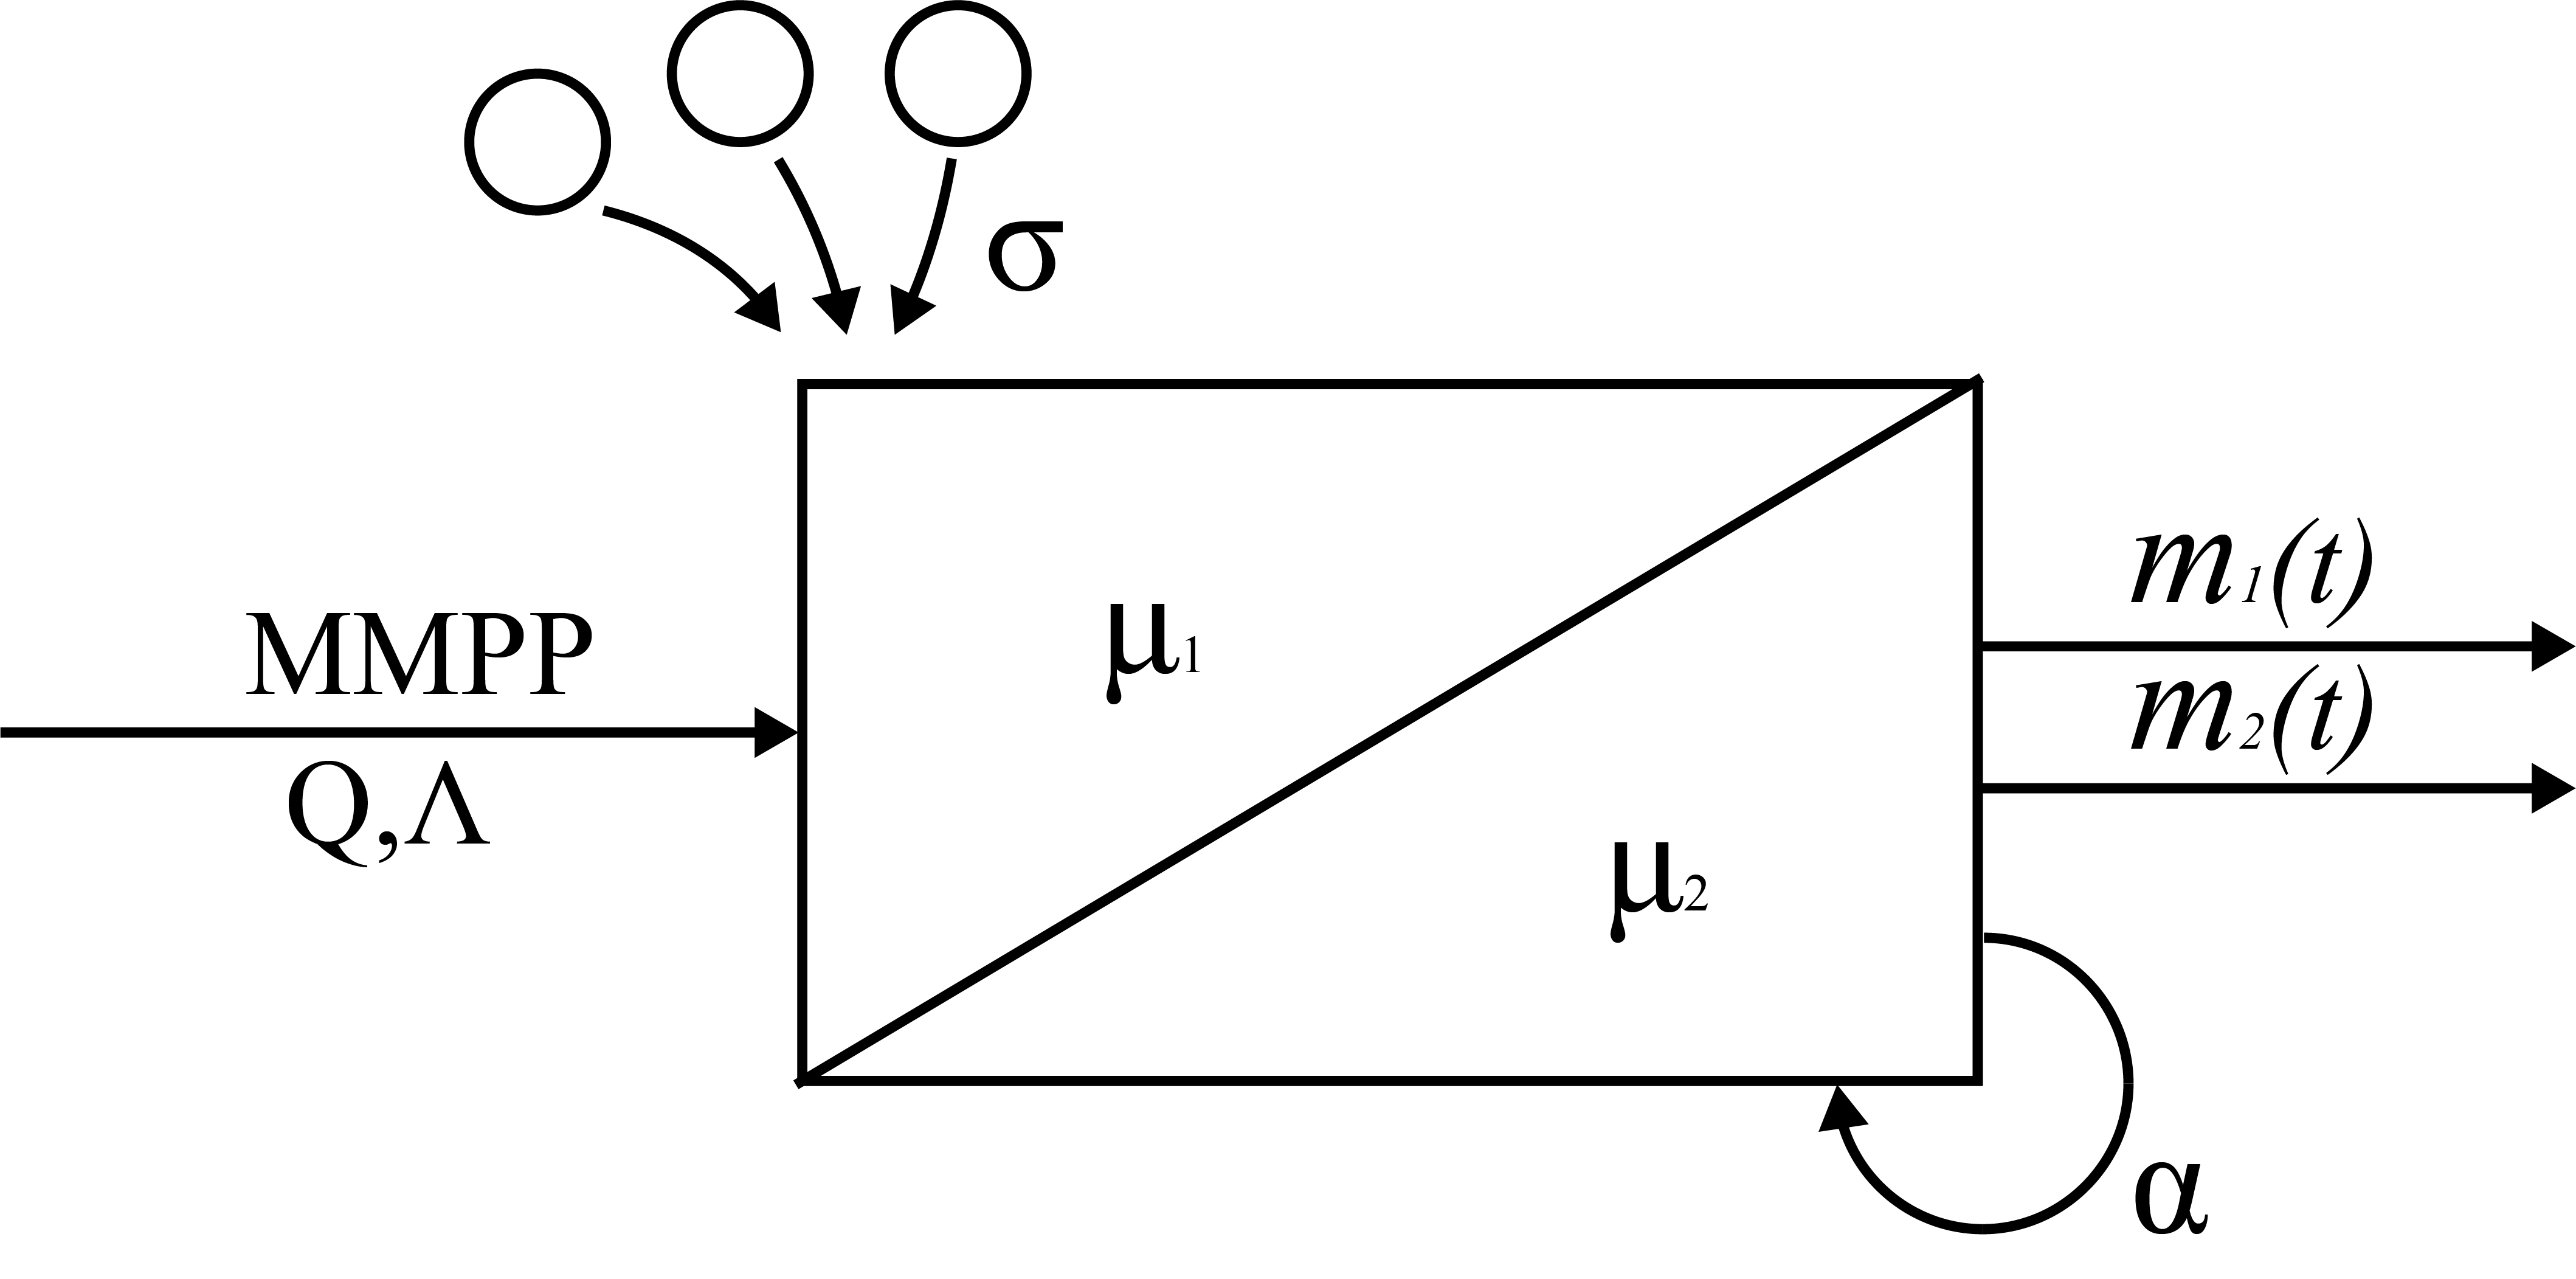
\includegraphics[scale=0.4]{RQ.png}
	\caption{Модель RQ--системы с повторными вызовами и обратной связью} \label{rq_system}
\end{figure}

Поскольку решение было получено при асимптотическом условии бесконечной задержки заявок в источнике повторных вызовов, требуется определить, при каких параметрах модели асимптотические результаты становятся недостоверными путем сравнения распределений вероятностей. Для это цели как раз отлично подходит имитационное моделирование.

В первую очередь, импортируем модуль q\_analysis, который и является разработанным программным комплексом. Он, в свою очередь, содержит модуль simulation для имитационного моделирования.
\begin{pyin}
	import q_analysis.simulation as q
\end{pyin}
Создадим модель и установим время моделирования, равное 1000000 условных единиц.
\begin{pyin} 
model = rq.Model()
model.set_time(0) 
model.set_end(100000)
model
\end{pyin}

\begin{pyout}
	Model{ time: 0, end : 1000000, event_queue_len : 0, num_components : 0, num_connections : 0 }
\end{pyout}

Далее добавим элементы модели (метод add\_producer). 

В модель добавятся следующие элементы: 
\begin{itemize}
	\item MMPP поток c матрицей $\Lambda$ следующего вида
		\begin{equation*}
			\Lambda =  \begin{bmatrix}
			1.0 & 0 &  0\\
			0 & 1.12 & 0\\
			0 & 0 &	0.45
			\end{bmatrix}
		\end{equation*} и матрицей $Q$
		\begin{equation*}
			Q =  \begin{bmatrix}
				-0.4 & 0.3 &  0.1\\
				0.5 & -0.6 & 0.1\\
				0.3 & 0.6 &	-0.9
			\end{bmatrix}
		\end{equation*};
	\item Орбита с экспоненциальной задержкой с интенсивностью $1$;
	\item Простейший поток с экспоненциальной задержкой с интенсивностью $1$ (будет использоваться как источник вызываемых заявок прибора);
	\item Обслуживающий прибор с экспоненциальным временем обслуживания входящих и вызываемых заявок с интенсивностью $1.15$.
\end{itemize}
Чтобы обращаться к элементам модели, им даются ярлыки - input, call, orbit, node.


\begin{pyin}
model.add_producer(rq.MMPPInput(
[1,1.12,0.45],
[[ -0.4, 0.3, 0.1],
[0.5,-0.6,0.1],
[0.3,0.6,-0.9]],0,0),"input")
model.add_producer(rq.SimpleInput(rq.ExponentialDelay(1),1,0),"call")
model.add_producer(rq.Orbit(rq.ExponentialDelay(1)),"orbit")
model.add_producer(rq.RqtNode(rq.ExponentialDelay(1.15),rq.ExponentialDelay(1.15)),"node")
print("Components:",model.components())
\end{pyin}

\begin{pyout}
	Components: {'node': RQTNode, 'orbit': Orbit, 'input': MMPP, 'call': SimpleInput}
\end{pyout}

Далее требуется соединить элементы модели при помощи маршрутизаторов. Для этого используется метод add\_connection. В параметрах указывается ранее заданный ярлык элемента модели, потом его вход или выход, функция возвращает ярлык нового соединения.

\begin{pyin}
	model.add_connection("input","out_slot","node","in_slot")
\end{pyin}
В данном случае мы указали входящий поток input и его выход out\_slot как источник заявок, и прибор node и его вход in\_slot как вход для приходящих заявок. Получим следующий ключ, описывающий соединение:
\begin{pyout}
'input:out_slot:node:in_slot'
\end{pyout}
С помощью полученной строки в последствии можно обращаться к соответствующими маршрутизатору при помощи метода reader\_at.

Далее добавляются остальные соединения. Для обслуживающего прибора маршрутизатор не будет сохранять в памяти обслуженные заявки. Это достигается использованием метода add\_hanging\_output\_noqueue:
\begin{pyin}
model.add_connection("call","out_slot","node","call_slot")
model.add_connection("node","orbit_append_slot","orbit","in_slot")
orb = model.add_connection("orbit","out_slot","node","orbit_slot")
output = model.add_hanging_output_noqueue("node","out_slot")
print("Connections",model.routers())
\end{pyin}

\begin{pyout}
Connections {
'onq:node:out_slot': Router{ queue_len: 0 },
'orbit:out_slot:node:orbit_slot': Router{ queue_len: 0 },
'node:orbit_append_slot:orbit:in_slot': Router{ queue_len: 0 },
'input:out_slot:node:in_slot': Router{ queue_len: 0 },
'call:out_slot:node:call_slot': Router{ queue_len: 0 }
}
\end{pyout}

Ярлыки маршрутизаторов называются по следующей схеме:
\begin{itemize}
	\item \textit{ ярлык выходного элемента :  имя выхода :  ярлык входного элемента : имя входа };
	\item для аккумулирующего входного маршрузитора (model.add\_hanging\_input) --- \textit{i :  ярлык входного элемента : имя входа}
	\item для аккумулирующего выходного маршрузитора (model.add\_hanging\_output) --- \textit{o :  ярлык выходного элемента : имя выхода}
	\item для выходного маршрузитора (model.add\_hanging\_output\_noqeuue) --- \textit{onq :  ярлык выходного элемента : имя выхода}
\end{itemize}

Добавим сбор статистики с интервалом в 20 условных единиц, что будет означать, что мы измеряем, сколько заявок было обслужено в системе за интервал времени, равный $20$:

\begin{pyin}
model.router_at(output).add_reader(rq.IntervalRouterReader(20),"stat")
model.router_at(output).readers()
\end{pyin}
\begin{pyout}
'stat': IntervalRouterReader
\end{pyout}

Теперь когда модель создана, нам требуется описать, как именно будет проходить ее запуск. Маршрутизация определяет топологию передачи заявок по системе, однако порядок взаимодействия элементов модели указывается в качестве отдельного алгоритма, так как, в зависимости от специфики задачи, он может варьироваться.
Процесс моделирования сводится к итеративному вызову метода produce у элементов модели с указанием в качестве параметра текущего времени моделирования. Результат работы produce (список моментов наступления предстоящих событий) передается в функцию модели aggregate для того, чтобы далее смещать время на нужные моменты. Именно порядок вызовов produce составляет алгоритм моделирования. В данно случае он будет следующим:
\begin{enumerate}
	\item генерация очередной заявки входящих потоком;
	\item возвращение заявок с орбиты;
	\item генерация очередной заявки источником вызываемых заявок;
	\item обслуживание заявки;
	\item сбор заявок, не сумевших захватить прибор.
\end{enumerate}

Построим цикл:
\begin{pyin}
from tqdm import tqdm
e = model.end()
with tqdm(total=int(e)) as pbar:     
t = c = 0
while True:
    c+=1 
    told = t
    t = model.next_step()
    pbar.update(t-told)
    model.aggregate(model.component_at("input").produce(t))
    model.aggregate(model.component_at("orbit").produce(t))
    model.aggregate(model.component_at("call").produce(t))
    model.aggregate(model.component_at("node").produce(t))
    model.aggregate(model.component_at("orbit").append(t))
    if model.is_done():
        break
print("Time: ",model.time())
print("Iters: ",c)
\end{pyin}

\begin{pyout}
Time:  1000000.0437646629
Iters:  21710021
\end{pyout}

По окончании моделировании мы можем проверить, какое распределение вероятностей числа обслуженных заявок за интервал $20$ получилось. Для этого обратимся к сборщику статистики маршрутизатора с ярлыком output и вызовем метод get\_distribution\_2d. Этот метод построит распределение вероятности числа обслуженных заявок двух типов --- входящих и вызванных.
\begin{pyin}
distr = model.router_at(output).reader_at('stat').get_distribution_2d()
import plotly.graph_objects as go
fig = go.Figure(data=[go.Surface(z=distr) ])

fig.update_traces(contours_z=dict(show=True, usecolormap=False,
highlightcolor="limegreen", project_z=True))

fig.update_layout(title='Model 2d distribution', autosize=False,
width=1000, height=1000,
margin=dict(l=65, r=50, b=65, t=90))

fig.show()
\end{pyin}

\begin{figure}[H]
	\centering
	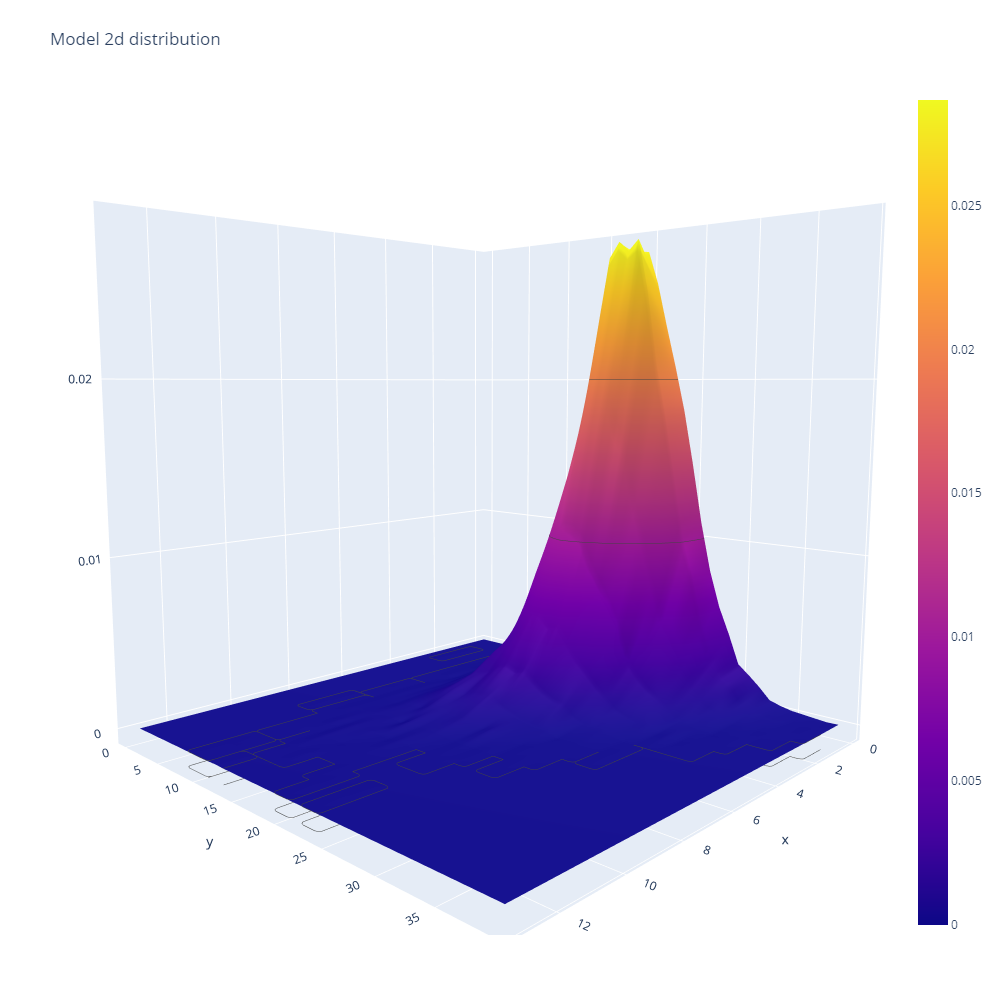
\includegraphics[scale=0.4,width=\textwidth]{model_2d_distr.png}
	\caption{Распределение числа обслуженных заявок по окончании имитационного моделирования} 
	\label{model_2d_distr}
\end{figure}

Далее получим характеристики выходящих процессов:

\begin{pyin} [rqtestchar]
print("Mean  called: {0},\nMean input: {1},\nVariation called: {2},\nVariation input: {3}".format(
model.router_at(output).reader_at('stat').get_mean_called(),
model.router_at(output).reader_at('stat').get_mean_input(),
model.router_at(output).reader_at('stat').get_variation_called(),
model.router_at(output).reader_at('stat').get_variation_input()))
\end{pyin}

\begin{pyout} 
Mean  called: 1.476929538590772,
Mean input: 19.793515870317407,
Variation called: 0.9226633215974042,
Variation input: 0.9463029320729057
\end{pyout}

В ячейке \ref{rqtestchar} представлены значения среднего числа обслуженных вызванных и входящих заявок, вариации числа обслуженных вызванных и входящих заявок соответственно.

Также мы можем экспортировать результаты в файл для работы в другой среде при помощи NumPy:
\begin{pyin} [rqtestchar]
np.array(distr).tofile('example_distr.txt')
\end{pyin}
Таким образом мы смогли получить характеристики выходящих процессов рассматриваемой модели системы и визуализировать полученный результат, используя ту же среду выполнения. Далее нам потребуется вычислить ранее полученные асимптотические результаты для этой модели системы и провести сравнение. Для указанной системы в программном пакете уже имеется алгоритм вычисления значений характеристической функции числа обслуженных заявок. Для начала импортируем его и модуль с утилитами, в котором содержится функция для подсчета расстояния Колмогорова

\begin{pyin} 
from q_analysis import rq_system as rq
from q_analysis import utils as u
\end{pyin}

Далее зададим такие же параметры системы как при моделировании и рассчитаем распределение:

\begin{pyin} 
Lambda = np.mat([[1, 0,   0],
[0,1.12, 0],
[0, 0,0.45]])

Q = np.mat([[ -0.4, 0.3, 0.1],
[0.5,-0.6,0.1],
[0.3,0.6,-0.9]])
alpha = 1
mu1 = 1.15
mu2 = 1.15

s = rq.RQSystem(mu1, mu2, Lambda, Q, alpha)
n = 43
m = 13
distr_asymp =    s.icfft2(n,m,20)
\end{pyin}

При визуализации полученного распределения на рисунке \ref{asymp_calc_example} видно, что оно практически полностью совпадает с распределением, полученным в результате имитационного моделирования (рисунок \ref{model_2d_distr})

\begin{figure}[H]
	\centering
	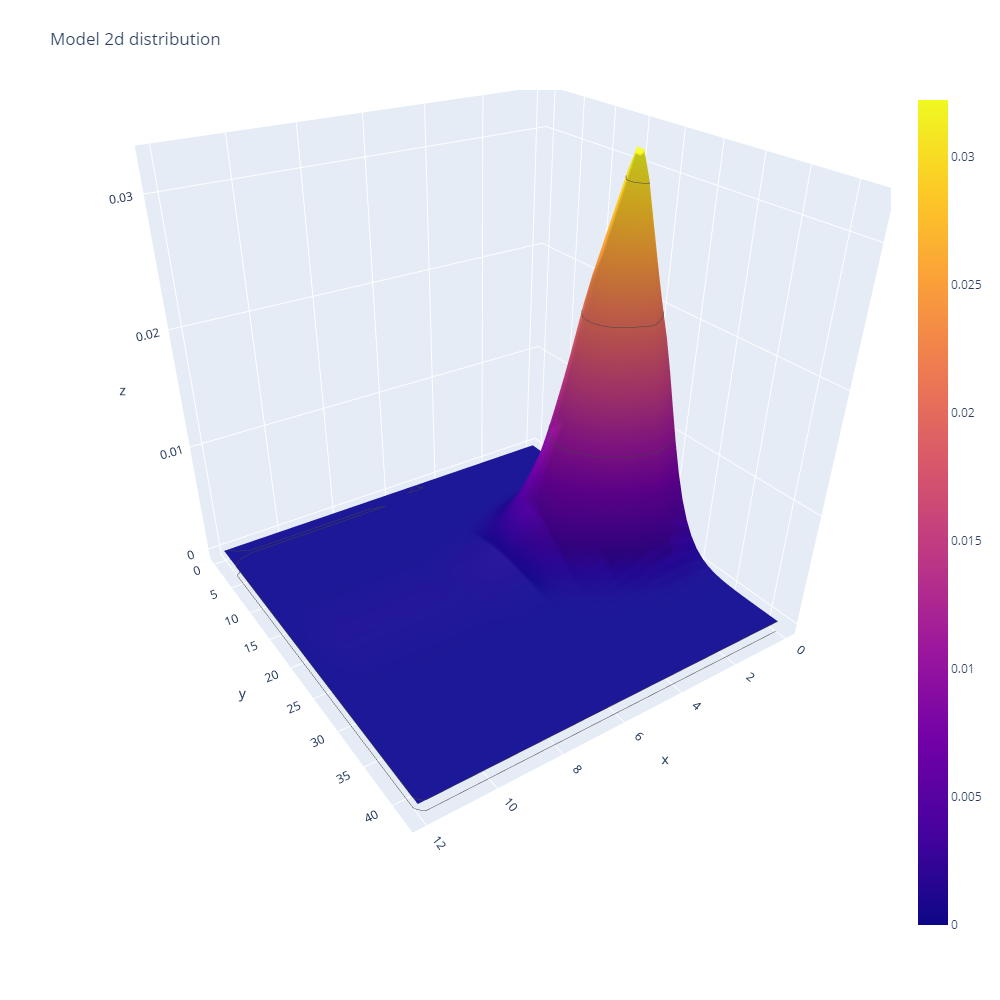
\includegraphics[scale=0.4,width=\textwidth]{asymp_calc_example.png}
	\caption{Распределение числа обслуженных заявок} 
	\label{asymp_calc_example}
\end{figure}

Для точечного сравнения распределений воспользуемся расстоянием Колмогорова:

\begin{pyin} 
u.k_distance2(distr,distr_asymp)
\end{pyin}

\begin{pyout} 
0.004355157840943953
\end{pyout}

Исходя из значения расстояния Колмогорова можно заключить, что при выбранных параметрах системы асимптотические результаты применимы, так как оно не превышает условного порога в $5\cdot 10^{-3}$.

Таким образом, мы можем использовать данный инструмент как для получения наблюдаемых численных характеристик при отсутствии аналитических решений, так и использовать его для сравнения с ними при их наличии посредством вычисления различных показателей и средств визуализации.

\subsection{Сбор и анализ данных о зависимости распределения заявок на орбите и времени ожидания}
В данном разделе рассматривается применение имитационной модели для решения задачи, требующей большой выборки данных. Суть ее составляет подтверждение наличия зависимости между числом заявок на орбите и временем ожидания заявки до ее обслуживания на приборе в системе, изображенной на рисунке \ref{rq_system}. Данная задача важна для понимания функционирования источника повторных вызовов и его влияния на эффективность обслуживания прибора. Поскольку требуется рассмотреть модель с различными параметрами орбиты и входящего потока, будет проводится ряд запусков, на основе которых в последствии будет производится поиск корреляции.

На число заявок на орбите, как и на время их обслуживания непосредственно влияют следующие параметры модели:
\begin{enumerate}
	\item интенсивность входящего потока;
	\item частота возращения заявок с орбиты;
	\item интенсивность обслуживания прибора.
\end{enumerate} 

Для конфигурации моделей интенсивность обслуживания будет зафиксирована, а интенсивность входящего потока и частота возвращения заявок с орбиты будет варьироваться.

Для хранения данных о моделировании и собираемых характеристиках работы моделей будем использовать словарь:
\begin{pyin} 
models = []
models_desc = []
\end{pyin}

Поскольку запусков будет много, будем запускать их в разных потоках для максимальной эффективности. Для этого объявим функции для генерации модели и запуска алгоритма. Это позволит нам использовать одну и ту же логику при параллельном запуске. Для упрощения задачи моделирования будет использоваться простейший входящий поток заявок, также зафиксируем интенсивность вызова заявок на значении 1. Для подсчета времени ожидания нам достаточно обновлять для каждой прошедшей заявки момент времени, в который он уходила с орбиты. В свою очередь для подсчета количества заявок на орбите нам потребуется учитывать, сколько заявок пришло на орбиту, и сколько ушло. Для этой цели прикрепим к маршрутизаторам, по котором заявки проходят через орбиту, счетчики TimeCounter.

\begin{pyin} 
def sim_task(i):
   t = c = 0
   while True:
      c+=1 
      t = models[i].next_step()
      models[i].aggregate(models[i].component_at("input").produce(t))
      models[i].aggregate(models[i].component_at("orbit").produce(t))
      models[i].aggregate(models[i].component_at("call").produce(t))
      models[i].aggregate(models[i].component_at("node").produce(t))
      models[i].aggregate(models[i].component_at("orbit").append(t))
      if models[i].is_done():
         print('#',end='')
         models[i].flush()
         break
\end{pyin}         

\begin{pyin}
def create_model(inp_i,orb_i,node_i):
model = rq.Model()
model.set_time(0) 
model.set_end(100000)

model.add_producer(rq.SimpleInput(rq.ExponentialDelay(inp_i),1,0),"input")
model.add_producer(rq.SimpleInput(rq.ExponentialDelay(1),1,0),"call")
model.add_producer(rq.Orbit(rq.ExponentialDelay(orb_i)),"orbit")
model.add_producer(rq.RqtNode(rq.ExponentialDelay(node_i),rq.ExponentialDelay(1.15)),"node")

model.add_connection("input","out_slot","node","in_slot")
model.add_connection("call","out_slot","node","call_slot")
orb_i = model.add_connection("node","orbit_append_slot","orbit","in_slot")
orb_o = model.add_connection("orbit","out_slot","node","orbit_slot")
output = model.add_hanging_output_noqueue("node","out_slot")

model.router_at(orb_i).add_reader(rq.AttemptCounter(),"attempt_count")
model.router_at(orb_i).add_reader(rq.TimeCounter(),"count")
model.router_at(orb_o).add_reader(rq.TimeCounter(),"count")
return model
\end{pyin}


Далее сгенерируем модели. Интенсивность входящего потока будет находится в границах $[0.1,1]$ c шагом $0.1$, орбита --- $[0.05,3]$ c шагом $0.1$, а интенсивность обслуживания в интервале $[1.6,2]$ с шагом $0.1$. Нижняя граница последнего интервала больше интенсивности входящего потока, так как условием стационарного режима для данной система является. Время моделирования установим в 200000 условных единиц, чего хватит для получения достоверных значений исследуемых характеристик. Для генерации моделей применим тройной вложенный цикл, итерации которого используют ранее установленные диапазоны:
\begin{pyin} 
input_intensity_range = np.arange(0.1, 1.0001, 0.1)
orbit_intensity_range = np.arange(0.05, 3.0001, 0.1)
node_intensity_range = np.arange(1.6001, 2.0001, 0.1)
m_index = 0

for inp in list(input_intensity_range):
   for orb in list(orbit_intensity_range):
      for nod in list(node_intensity_range):
         m = {}
         m['model_index'] = m_index
         m_index+=1
         m['input_intensity'] = inp
         m['orbit_intensity'] = orb
         m['node_intensity'] = nod
         models_desc.append(m)
         models.append(create_model(inp,orb,nod))
\end{pyin}

Для каждого запуска будем хранить заданные параметры в словаре, который в последствии также наполнится другими данными о моделировании, что позволит нам создать полноценную выборку для анализа:

\begin{pyin}
for m in models_desc:
   print(m)
\end{pyin}

\begin{pyprint}
{'model_index': 0, 'input_intensity': 0.8, 'orbit_intensity': 0.8, 'node_intensity': 1.55}
{'model_index': 1, 'input_intensity': 0.8, 'orbit_intensity': 0.8, 'node_intensity': 1.65}
{'model_index': 2, 'input_intensity': 0.8, 'orbit_intensity': 0.8, 'node_intensity': 1.75}
{'model_index': 3, 'input_intensity': 0.8, 'orbit_intensity': 0.8, 'node_intensity': 1.85}
...
\end{pyprint}

Итак, получилось 1500 моделей с различными параметрами. Запустим их в 12-ти процессах при помощи объекта ThreadPool из встроенной библиотеки Python multiprocessing \cite{multiproc}, предназначенной для конкурентной работы:
\begin{pyin}
print('#'*(len(models)-1))
from multiprocessing.pool import ThreadPool
r = list(range(0,len(models)-1))
with  ThreadPool(processes=12) as p:
   p.map(sim_task, r )
\end{pyin}

Для последующего анализа рассчитаем ряд показателей:
\begin{itemize}
	\item среднее число заявок на орбите;
	\item среднее время ожидания заявки до обслуживания;
	\item коэффициент вариации числа заявок на орбите;
	\item среднеквадратическое отклонение числа заявок на орбите;
	\item среднеквадратическое отклонение времени ожидания заявок;
	\item коэффициент вариации времени ожидания заявок.
\end{itemize}

Пример полученный таблицы с характеристиками:

\begin{table}[H] 
	\centering
	\caption{Показатели для оценки зависимости числа заявок на орбите и времени ожидания заявки}
	\label{sim_result_1}
\begin{tabular}{|c|c|c|c|c|c|c|c|c|c|c|c|c|c|} 
\hline
$\lambda$ & $\mu$   &  $\sigma$ &  os\_mean &   wt\_mean &      os\_std &     wt\_std &       os\_var &     wt\_var \\
\hline
0.100 &           1.600 &           0.050 &    2.044 &   20.395 &   1.487 &  35.386 &   0.728 &   1.735 \\
\hline
0.100 &           1.700 &           0.050 &    2.035 &   20.144 &   1.484 &  34.628 &   0.729 &   1.719 \\
\hline
0.100 &           1.800 &           0.050 &    1.994 &   20.198 &   1.489 &  34.612 &   0.747 &   1.714 \\
\hline
0.100 &           1.900 &           0.050 &    1.969 &   19.485 &   1.480 &  33.644 &   0.752 &   1.727 \\
\hline
0.100 &           2.000 &           0.050 &    1.998 &   19.317 &   1.466 &  33.433 &   0.734 &   1.731 \\
\hline
0.100 &           1.600 &           0.150 &    0.734 &    7.293 &   0.898 &  12.226 &   1.223 &   1.676 \\
\hline
0.100 &           1.700 &           0.150 &    0.688 &    7.049 &   0.861 &  12.026 &   1.252 &   1.706 \\
\hline
0.100 &           1.800 &           0.150 &    0.688 &    7.028 &   0.871 &  11.913 &   1.267 &   1.695 \\
\hline
0.100 &           1.900 &           0.150 &    0.689 &    6.956 &   0.871 &  11.813 &   1.264 &   1.698 \\
\hline
0.100 &           2.000 &           0.150 &    0.689 &    6.903 &   0.866 &  11.907 &   1.258 &   1.725 \\
\hline
0.100 &           1.600 &           0.250 &    0.436 &    4.349 &   0.686 &   7.321 &   1.574 &   1.683 \\
\hline
0.100 &           1.700 &           0.250 &    0.450 &    4.524 &   0.700 &   7.633 &   1.557 &   1.687 \\
\hline
0.100 &           1.800 &           0.250 &    0.440 &    4.411 &   0.691 &   7.292 &   1.569 &   1.653 \\
\hline
0.100 &           1.900 &           0.250 &    0.428 &    4.349 &   0.681 &   7.338 &   1.590 &   1.687 \\
\hline
0.100 &           2.000 &           0.250 &    0.429 &    4.320 &   0.684 &   7.223 &   1.593 &   1.672 \\
\hline
\end{tabular}
\end{table}

После того, как выборка создана, рассмотрим распределение каждой из характеристик. На рисунке \ref{orbit_size_plot} представлены распределения вероятностей числа заявок на орбите во время моделирования. Как видно, для некоторых наборов параметров наблюдаются скопления похожих распределений. Также видно, что с изменением параметров математическое ожидание заметно смещается:

\begin{figure}[H]
	\centering
	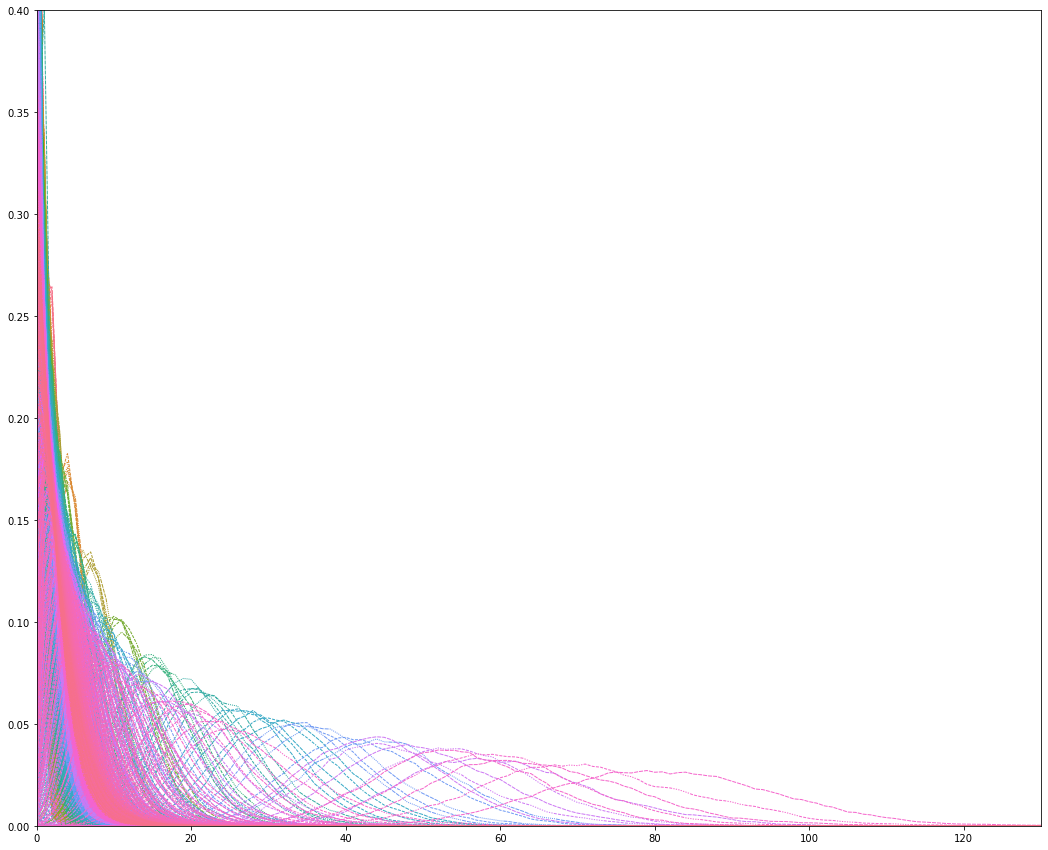
\includegraphics[scale=0.4,width=\textwidth]{orbit_size_plot_all.png}
	\caption{Распределения числа заявок на орбите} 
	\label{orbit_size_plot_all}
\end{figure}

На рисунке \ref{wait_time_plot} представлены распределения времени до обслуживания заявки:

\begin{figure}[H]
	\centering
	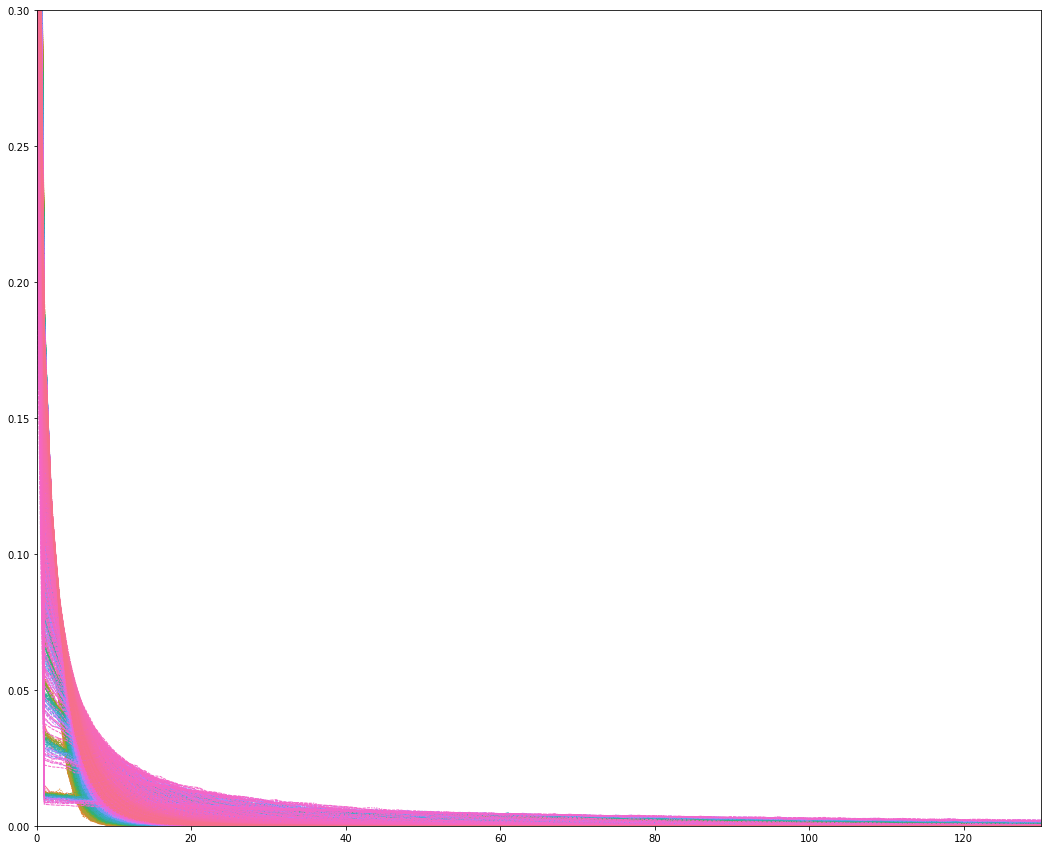
\includegraphics[scale=0.4,width=\textwidth]{wait_time_plot_all.png}
	\caption{Распределения числа заявок на орбите} 
	\label{wait_time_plot_all}
\end{figure}

Для того, чтобы выявить зависимости между показателями воспользуемся графиками рассеяния, где каждому наблюдению будет соответствовать точка на декартовой плоскости. По каждой из осей отложены рассматриваемые показатели, и в случае, если между ними имеется корреляционная зависимость, на диаграмме это будет представлено в виде определенной закономерности, согласно которой расположены точки. В случае положительной корреляции оба значения будут расти и наоборот:
\begin{figure}[H]
	\centering
	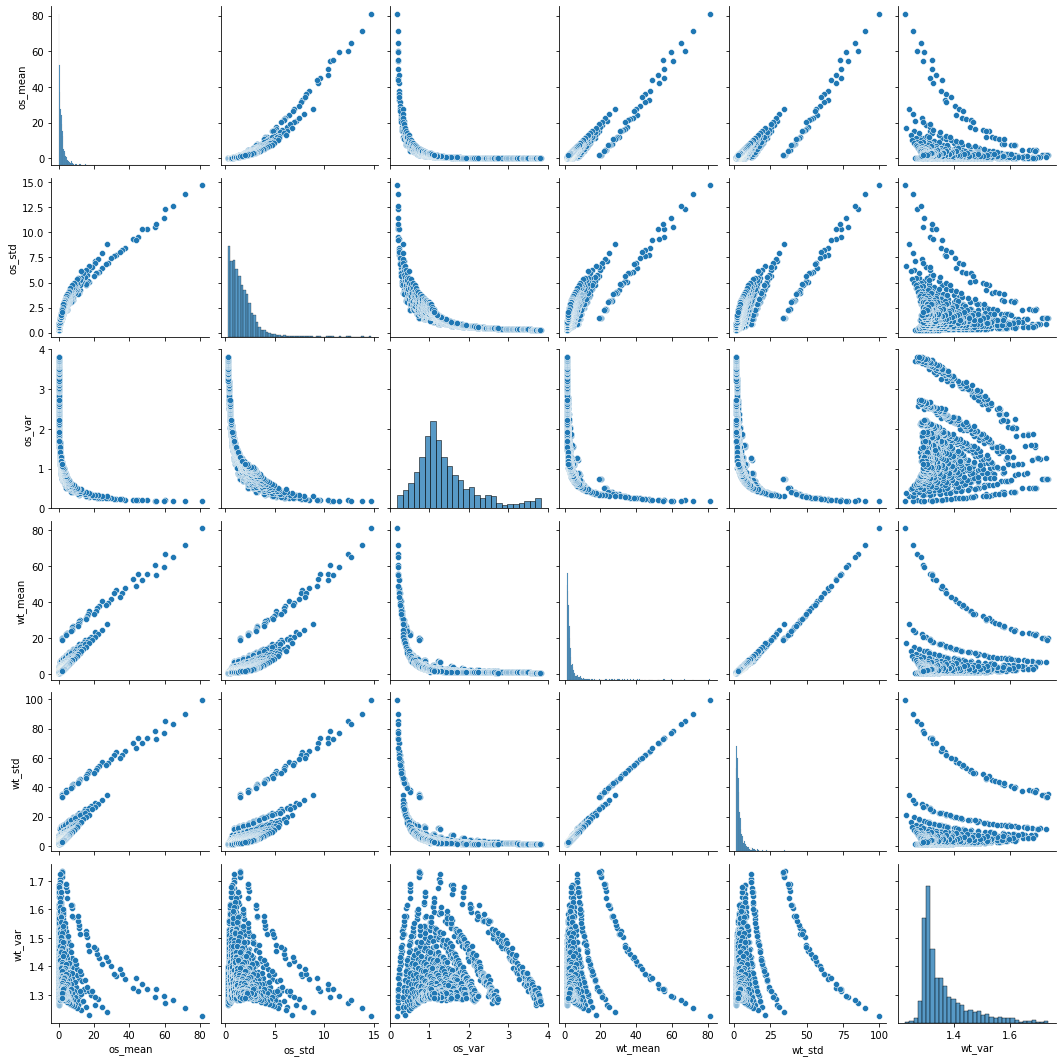
\includegraphics[scale=0.4,width=\textwidth]{pairplot_all.png}
	\caption{График рассеяния} 
	\label{os_wt_pairplot_all}
\end{figure}

Для всех метрик, касающихся размера орбиты установлен префикс os\_, для метрик времени ожидания заявкой обслуживания --- wt\_. Как видно из графика рассеяния (например пара os\_var --- wt\_mean) зависимость между характеристиками есть. Это также можно видеть на паре os\_mean --- wt\_std или os\_mean -- wt\_mean, где очевиден линейный ее характер. Однако также на графике видны некие разрывы в наблюдений. Причиной тому может быть способ задания параметров моделей, при котором не были учтены некоторые интервалы значений, в результате не попавшие в наблюдения. Чтобы более ясно увидеть зависимость между двумя исследуемые характеристиками проведем еще два численных эксперимента: в первом случае будем варьировать только интенсивность обращения с орбиты, во втором --- интенсивность входящего потока. При таком подборе параметров получаемые наблюдения будут более гладкими и пригодны к анализу.

Также в рамках проводимых экспериментов воспользуемся несколько иным методом проведения параллельных вычислений. Он заключается в выделении кода, отвечающего за непосредственный запуск имитационной модели, в отдельный скрипт, что позволить его запускать при помощи интерпретатора Python в качестве отдельного процесса. Данный подход имеет два основных преимущества: во--первых, Python снабжен механизмом под названием Global Interpeter Lock или GIL \cite{gil}, который предотвращает использование интерпретатора за раз больше чем в одном процессе. При использовании вложенных процессов же будет запущен отдельный интерпретатор на каждый процесс. Данное ограничение может являться проблемой при параллельном запуске, так как фактически программа будет работать в однопоточном режиме. Во--вторых, при данном подходе появляется возможность удобно контролировать объем потребляемых программой вычислительных ресурсов (оперативная память и время процессора). Это является важным аспектом при проведении моделирования, например, на домашнем компьютере, не обладающим достаточным количеством ресурсов для запуска большого количество процессов за раз.

Реализация данного подхода представлена ниже:

\begin{pyin} [subprocess_example]
import subprocess
import json
import numpy as np
res = []
procs = []
input_intensity_range = np.arange(0.1, 1.0001, 0.1)
orbit_intensity_range = np.arange(0.05, 3.0001, 0.1)
node_intensity_range = np.arange(1.6001, 2.0001, 0.1)

completed_count = 0
m_index = 0
for inp in list(input_intensity_range):
   for orb in list(orbit_intensity_range):
      for nod in list(node_intensity_range):
         procs.append(subprocess.Popen(' '.join(['python','run.py',str(inp),str(orb),str(nod)]),shell=True))
         m_index +=1
         if m_index>100:
            procs[0].wait()
            m_index-=1
            procs.pop(0)
            completed_count+=1
            print(f'Completed: {completed_count}',end="\r",flush=True)


for p in procs:
   p.wait()
   completed_count+=1
   print(f'Completed: {completed_count}',end="\r",flush=True)
\end{pyin}

В ячейке \ref{subprocess_example} в тройном вложенном цикле в качестве вложенного процесса запускается скрипт run.py для каждого набора параметров. В нем содержится вся логика моделирования, а также код для сохранения результатов в требуемый формат (в данном случае используется JSON). Переменная m\_index позволяет нам учитывать количество запущенных процессов. При каждом запуске мы инкрементируем ее, при каждом завершении процесса - декрементируем. А для ограничения количества запущенных процессов мы можем сравнивать значение m\_index на каждой итерации с заданным максимальным числом запущенных процессов (в данном случае 100). В случае, если число запущенных процессов достигло порога, мы вызываем метод wait у объекта процесса, тем самым дожидаясь пока один из процессов завершится, чтобы мы могли запустить новый. Таким образом, всегда будет запущено лишь максимально допустимое число процессов. Определение нужного значения порога определяется эмпирически, например посредством запуска одной модели и замером потребляемой памяти при помощи встроенного пакета psutil \cite{psutil}.


\begin{pyin}  [res_example]
from os import listdir
from os.path import isfile, join
import pandas as pd

res = []

for f in [f for f in listdir('results/') if isfile(join('results/', f))]:
   with open(f'results/{f}','r',encoding='utf-8') as ff:
   res.append(json.load(ff))

df = pd.DataFrame(res)
\end{pyin}

По окончании моделирования мы можем прочитать все файлы в директории с результатами (ячейка \ref{res_example}) и на их основе, например, создать объект DataFrame, позволяющий работать с данными в табличном виде.

Описанным методом были получены результаты для двух дополнительных экспериментов:
\begin{itemize}
	\item $\sigma$ варьируется в интервале $[0.05,10]$ с шагом $0.05$. $\lambda$ и $\mu$ зафиксированы на значениях $1$ и $1.5$ соответственно. Проведено 100 запусков;
	\item $\lambda$ варьируется в интервале $[0.1,1.7]$ с шагом $0.01$. $\sigma$ и $\mu$ зафиксированы на значениях $1$ и $1.8$ соответственно. Проведено 160 запусков.
\end{itemize}

Для иллюстрации влияния параллельного моделирования на производительность были проведены 100 запусков для первого набора параметров с использованием алгоритма, изложенного в ячейке \ref{subprocess_example}: в первом случае, когда модели запускались последовательно, общее время моделирования составило 16 минут 4 секунды, во втором, когда было запущено до 10 моделей параллельно --- 4 минуты 29 секунд. 

В итоге были получены более пригодные к анализу выборки, на основе которых построены графики рассеяния \ref{os_wt_pairplot_sigma} и \ref{os_wt_pairplot_l}:

\begin{figure}[H]
	\centering
	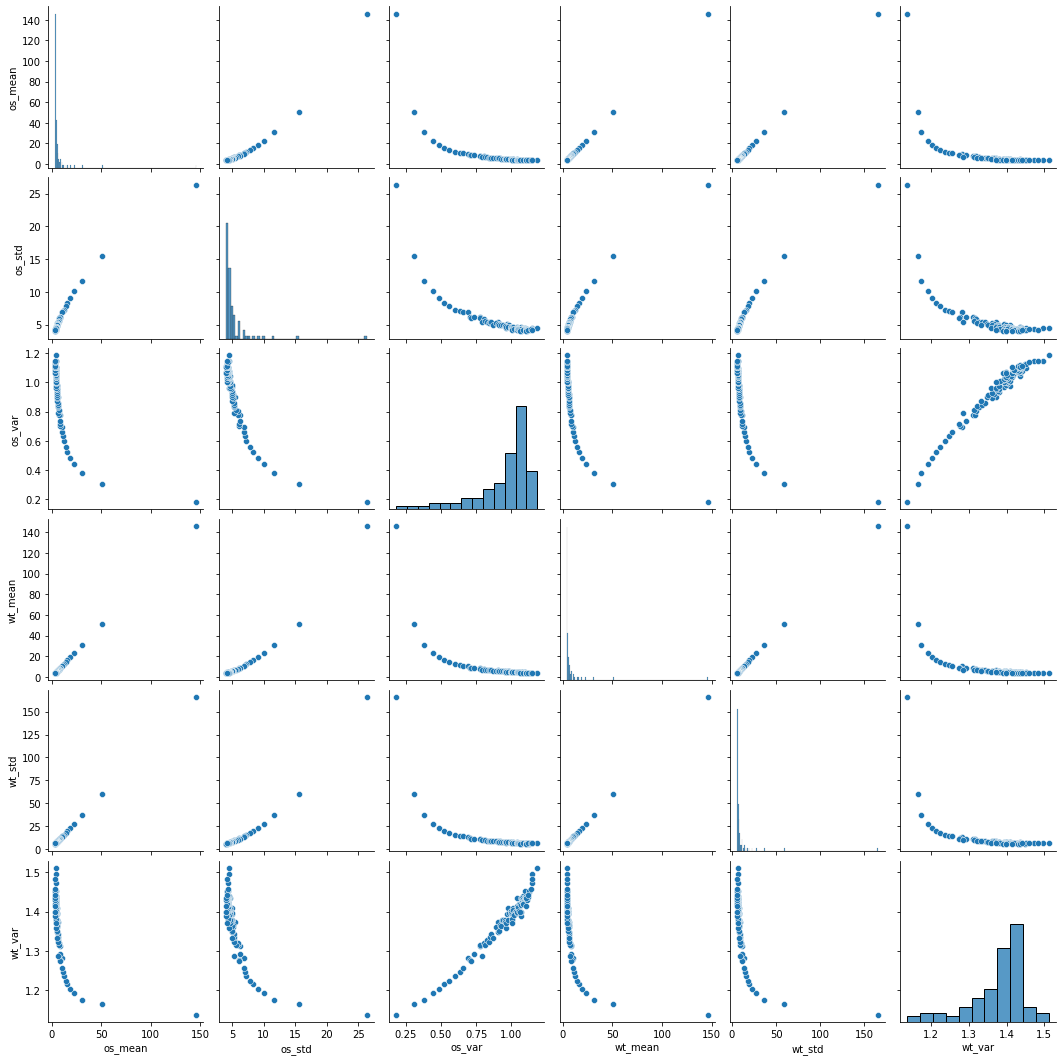
\includegraphics[scale=0.4,width=\textwidth]{pairplot_sigma.png}
	\caption{График рассеяния при фиксированном $\sigma$} 
	\label{os_wt_pairplot_sigma}
\end{figure}

\begin{figure}[H]
	\centering
	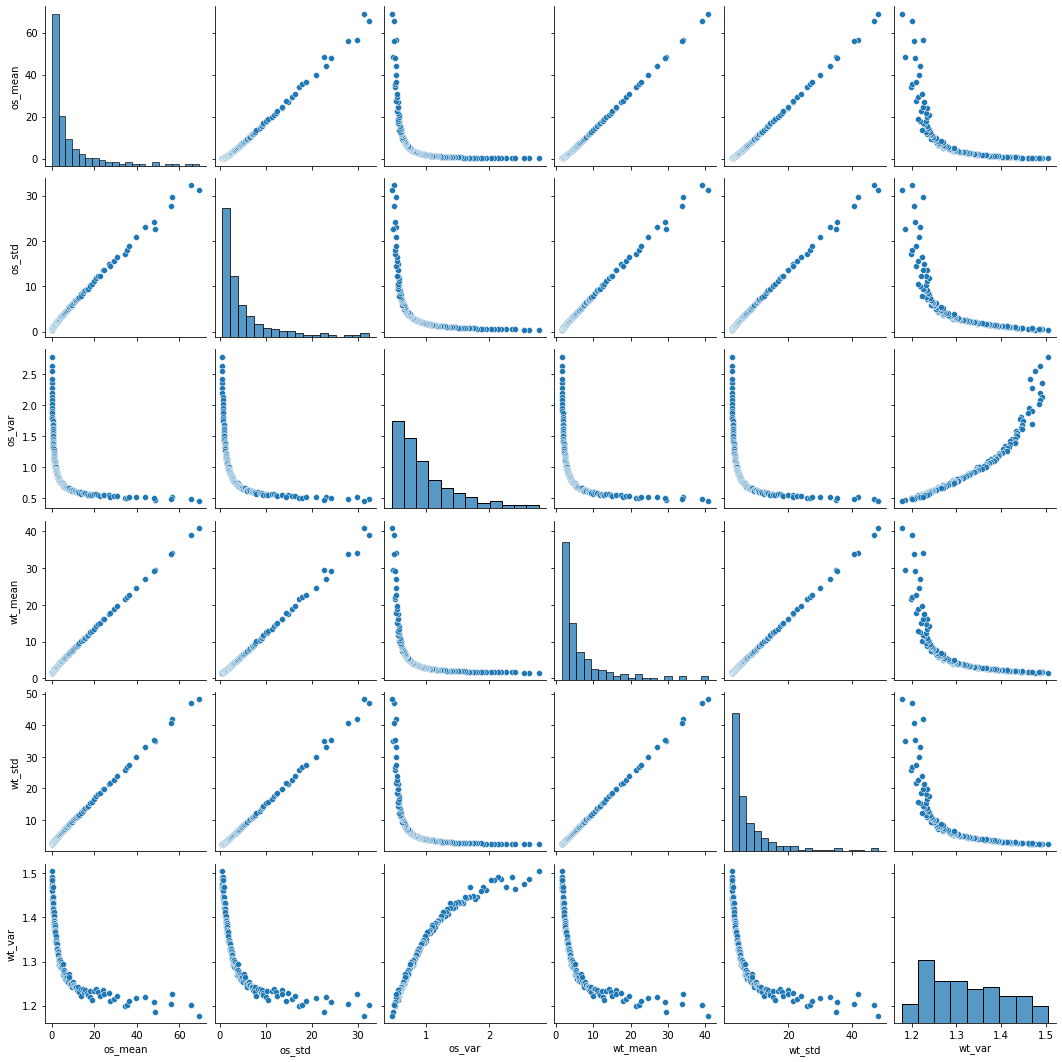
\includegraphics[scale=0.4,width=\textwidth]{pairplot_l.png}
	\caption{График рассеяния при фиксированном $\lambda$} 
	\label{os_wt_pairplot_l}
\end{figure}

Как видно из полученных наблюдений, исследуемые характеристики явно коррелируют; это можно заключить основываясь на паре os\_mean --- wt\_mean и os\_std --- wt\_std, где наблюдается линейная зависимость между величинами.

\begin{figure}[H]
	\centering
	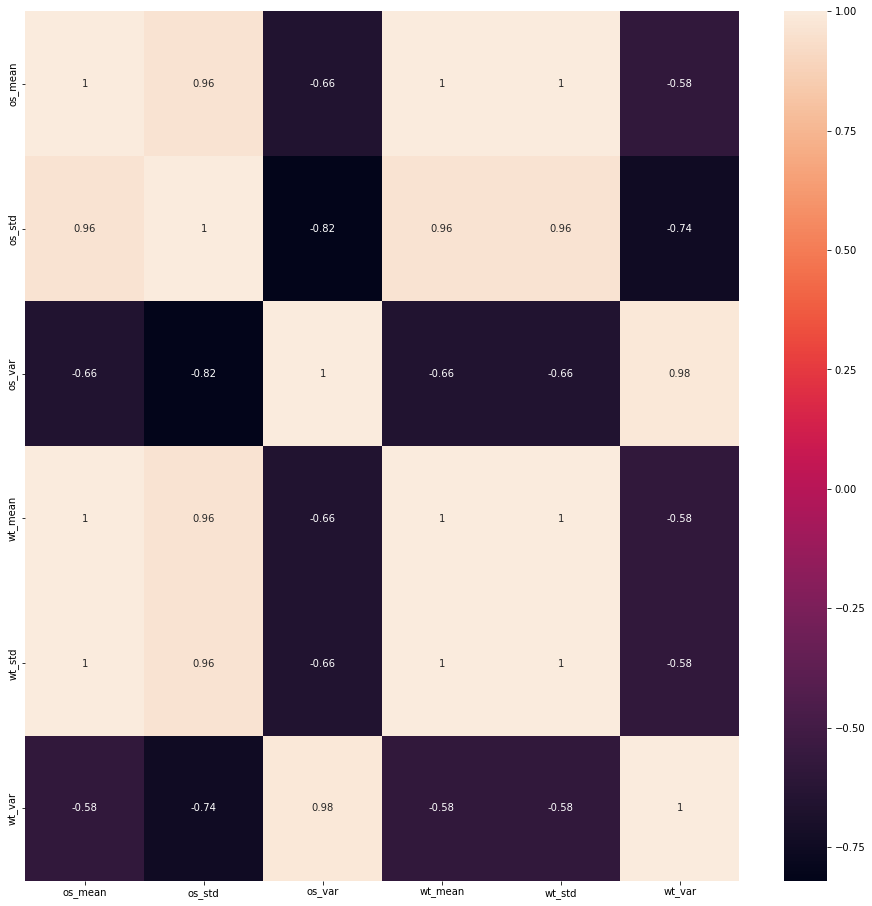
\includegraphics[scale=0.4,width=\textwidth]{corr_plot_sigma.png}
	\caption{Корреляционная карта числа метрик числа заявок на орбите и времени их ожидания до обслуживания} 
	\label{os_wt_corr_map}
\end{figure}

Корреляционная карта \ref{os_wt_corr_map} подтверждает произведенные ранее наблюдения на графике рассеяния --- между вариацией числа заявок на орбите (os\_var) и математическим ожиданием времени их ожидания наблюдается отрицательная зависимость --- $-0.66$. Аналогичные значения вычислены и для других метрик методом Пирсона.

На данном этапе, имея полученные данные о запусках 1760-и моделей с различными параметрами, можно заключить, что между распределением числа заявок на орбите и временем ожидания заявки до обслуживания имеется корреляционная связь.

\subsection{Апробация машинного обучения}
В данной главе описывается апробирование подхода к анализу систем массового обслуживания при помощи машинного обучения, а именно --- предсказывание коэффициента вариации длин интервалов между моментами покидания заявок системы. Данный метод широко используется во многих других областях науки и является универсальным: подходит для задач регрессии, временных рядов, а также классификации и кластеризации \cite{libbrecht2015machine,shinde2018review,soofi2017classification}. В теории массового обслуживания также есть примеры исследования, в которых успешно используется машинное обучение \cite{ojeda2021learning,xue2016scheduling,balla2018reliability}.

В первую очередь, в данном разделе показано, что разработанный программный пакет позволяет проводить крупномасштабные численные эксперименты, результаты которых достаточны, чтобы создать обучающую выборку и на ее основе обучить ряд моделей машинного обучения, способных предсказывать численные характеристики работы модели системы. Благодаря этому для ряда решаемых в теории массового обслуживания задач становятся доступны новые методы исследования.

\subsubsection{Разведочный анализ}
В данном случае машинное обучение будет использоваться для решения задачи регрессии. Для этой цели, при помощи ранее описанных инструментов, было проведено около 286 тысяч запусков имитационной модели при различных параметрах входящего потока, орбиты и обслуживающего прибора для создания выборки, на основе которой и будет решена задача.

Исходная выборка имеет 9 признаков:
\begin{enumerate}
	\item elapsed --- время работы имитационной модели в секундах. Данный признак был добавлен в утилитарных целях, в частности, для последующей оптимизации работы модели при нестандартных параметрах. Действительное число.
	\item mean\_input --- среднее число обслуженных заявок входящего потока за интервал моделирования. Действительное число.
	\item var --- коэффициент вариации длин интервалов между моментами наступления событий во входящем потоке. Действительное число.
	\item alpha --- интенсивность вызова заявок прибором ($\alpha$). Действительное число.
	\item lg --- интенсивность входящего потока. Действительное число.
	\item mu1 --- интенсивность обслуживания входящих заявок ($\mu_1$). Действительное число.
	\item mu2 --- интенсивность обслуживания вызванных заявок ($\mu_2$). Действительное число.
	\item sigma --- интенсивность обращений заявок с орбиты ($\sigma$). Действительное число.
	\item var\_input --- коэффициент вариации выходящего процесса. Действительное число. Является целевой переменной для предсказаний.
\end{enumerate}

Все признаки имеют 270420 (часть экспериментов выбыли из-за превышения временного лимита на выполнение) ненулевых значений и распределены следующим образом	
\begin{table}[H]
	\centering
	\caption{Распределение признаков}
	\label{table_feature_distr}
	\begin{tabular}{|l|l|l|l|l|l|l|l|l|l|l|}
		\hline
		& elapsed & mean\_input & var\_input &     alpha &        lg &       mu1 &       mu2 &     sigma &       var \\
		\hline
		mean & 7.36 &       5.52 & 1.11 &      1.26 &      1.90 &      2.97 &      2.71 &      1.41 &      1.32 \\
		\hline
		std & 23.16 &       5.43 & 0.20 &      0.91 &      0.68 &      0.66 &      0.81 &      0.86 &      0.31 \\
		\hline
		min & 0.01 &       0.00 & 0.71 &      0.00 &      1.00 &      1.20 &      1.00 &      0.01 &      1.00 \\
		\hline
		10\% & 0.79 &       0.57 & 0.93 &      0.20 &      1.00 &      2.00 &      1.40 &      0.21 &      1.05 \\
		\hline
		20\% & 1.29 &       1.15 & 1.00 &      0.40 &      1.20 &      2.40 &      2.00 &      0.61 &      1.09 \\
		\hline
		30\% & 1.74 &       1.82 & 1.01 &      0.60 &      1.40 &      2.60 &      2.20 &      0.81 &      1.14 \\
		\hline
		40\% & 2.19 &       2.66 & 1.03 &      0.80 &      1.60 &      2.80 &      2.60 &      1.21 &      1.18 \\
		\hline
		50\% & 2.70 &       3.70 & 1.06 &      1.20 &      1.80 &      3.00 &      2.80 &      1.41 &      1.24 \\
		\hline
		60\% & 3.34 &       5.03 & 1.09 &      1.40 &      2.00 &      3.20 &      3.00 &      1.81 &      1.30 \\
		\hline
		70\% & 4.32 &       6.77 & 1.14 &      1.80 &      2.20 &      3.40 &      3.20 &      2.01 &      1.37 \\
		\hline
		80\% & 6.21 &       9.23 & 1.20 &      2.00 &      2.60 &      3.60 &      3.60 &      2.41 &      1.48 \\
		\hline
		90\% & 11.76 &      13.25 & 1.32 &      2.60 &      2.80 &      3.80 &      3.80 &      2.61 &      1.67 \\
		\hline
		95\% & 22.72 &      16.87 & 1.46 &      3.00 &      3.20 &      3.80 &      3.80 &      2.81 &      1.87 \\
		\hline
		99\% & 104.70 &      24.02 & 1.86 &      3.40 &      3.40 &      3.80 &      3.80 &      2.81 &      2.45 \\
		\hline
		max & 419.53 &      35.89 & 5.99 &      3.60 &      3.60 &      3.80 &      3.80 &      2.81 &      8.19 \\
		\hline
	\end{tabular}
\end{table}
На основе сводки из таблицы \ref{table_feature_distr} можно заметить, что в среднем время моделирования занимало 7.36 секунд, половина экспериментов была запущена с интенсивностью входящего потока 1.8, а максимальный коэффициент вариации выходящего процесса составил 8.19.



На данном этапе мы можем избавиться от признаков, которые не будут участвовать в обучении модели: mean\_input и elapsed. Для оставшихся признаков построим графики рассеяния \cite{cox2007pairplot}. Данные диаграммы полезны для отображения многомерных данных, как в данном случае. С их помощью можно определить потенциальные взаимосвязи между количественными переменными.
\begin{figure}[H]
	\centering
	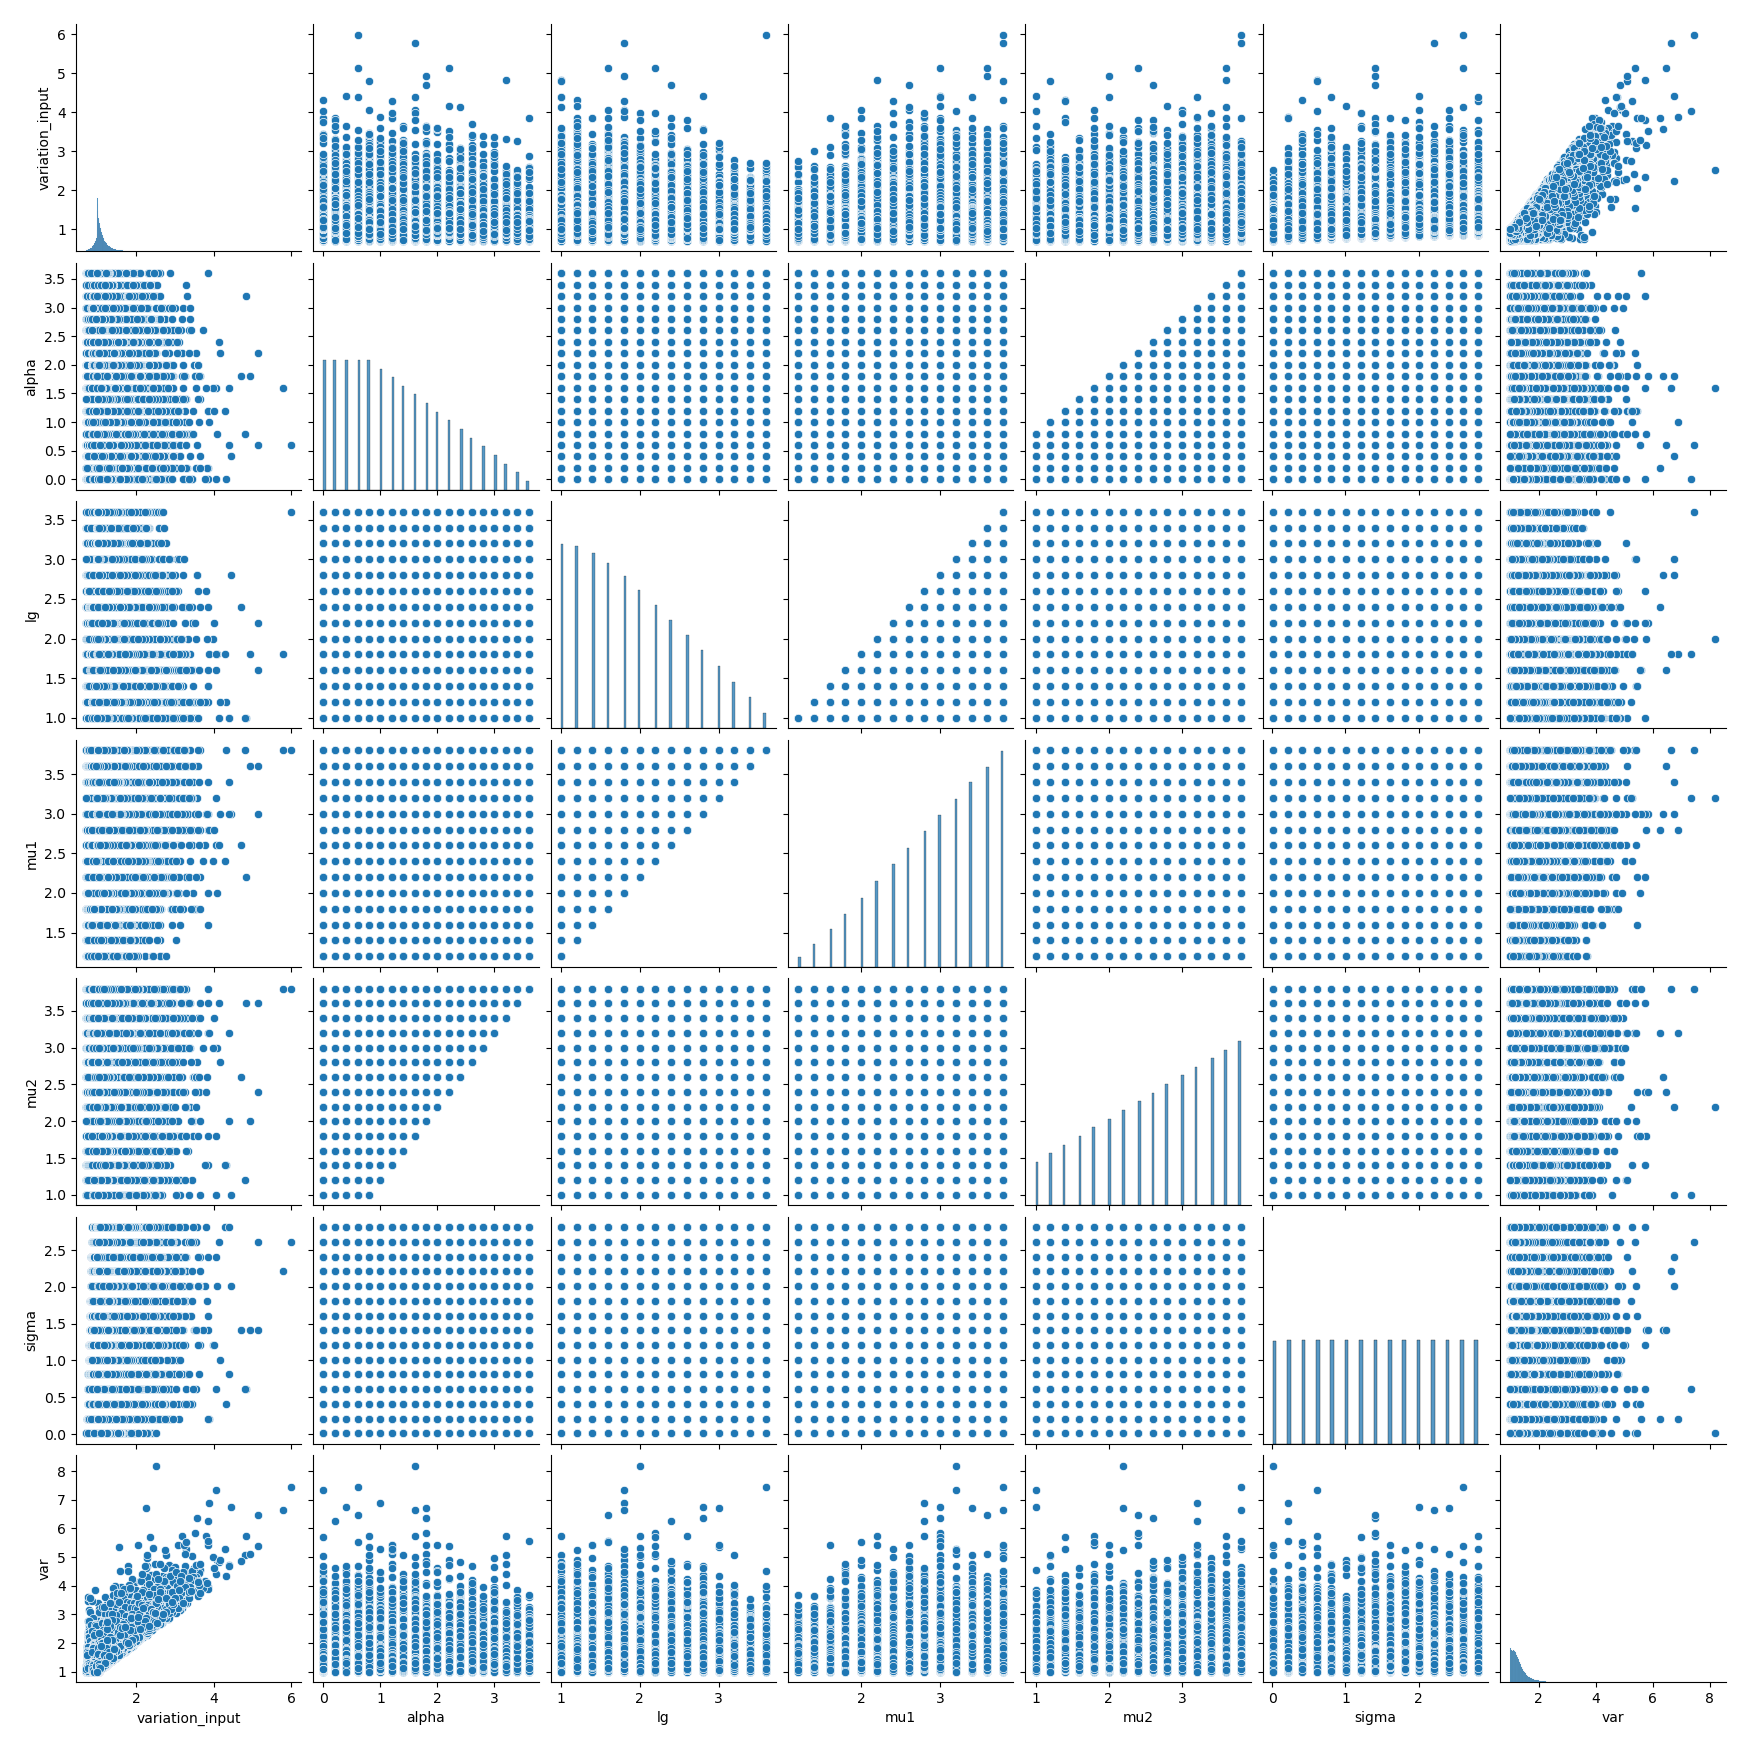
\includegraphics[scale=0.8,width=\textwidth]{pairplot.png}
	\caption{Графики рассеяния признаков}
	\label{pairplot}
\end{figure}
\clearpage
На графике рассеяния \ref{pairplot} видно, что явную связь имеют коэффициент вариации входящего потока (var) и коэффициент вариации выходящего процесса (var\_input). Для более точного определения зависимостей построим для признаков тепловую карту коэффициента корреляции Пирсона
\begin{figure}[H]
	\centering
	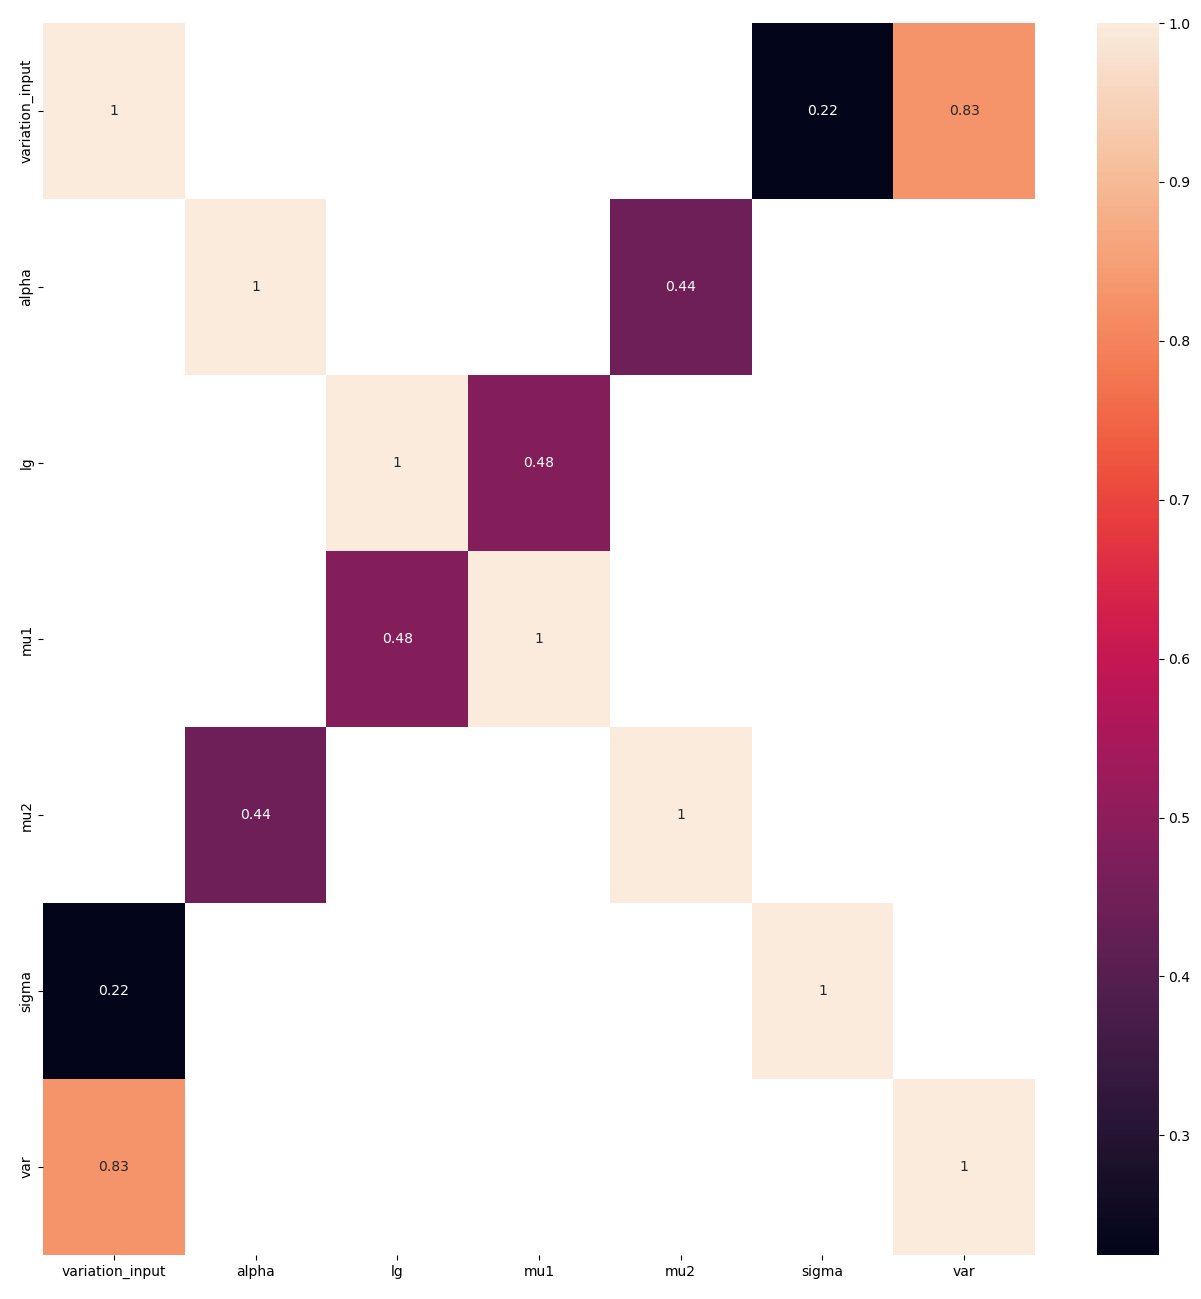
\includegraphics[scale=0.8,width=\textwidth]{pearson_heatmap.png}
	\caption{Тепловая карта корреляции признаков}
	\label{pearson_heatmap}
\end{figure}
На рисунке \ref{pearson_heatmap} можно наблюдать логичную корреляцию таких признаков, как интенсивность обслуживания входящих заявок (mu1) и интенсивность входящего потока (lg), а также интенсивность обслуживания вызванных заявок (mu2) и интенсивность их вызова (alpha). Для целевой переменной же можно наблюдать ранее выявленную корреляцию с коэффициентом вариации входящего потока и интенсивностью обращения заявок с орбиты (sigma), что так же ожидаемо, поскольку задержка заявок на орбите влияет на пропускную способность прибора.

\subsubsection{Построение предсказательных моделей}
Для настройки и обучения предсказательных моделей используется язык Python и библиотека для ансамблевого машинного обучения scikit-learn \cite{hackeling2017mastering}. Ансамблевые методы машинного обучения являются мощным и в то же время простым для понимая инструментом анализа данных. Он представляет собой метод обучения, где несколько моделей обучаются решению одной и той же задачи и объединяются для получения наиболее точных результатов. Ключевое преимущество такого метода заключается в том, что результат работы нескольких моделей будет иметь большую точность, чем результат только одной модели.
Будут обучены и протестированы следующие модели:
\begin{itemize}
	\item LinearRegression --- реализация метода наименьших квадратов. Будет использована для проверки правильности выборки и сравнения с другими, более сложными методами.
	\item RandomForest \cite{rigatti2017random} --- алгоритм, основывающийся на ансамбле решающих деревьев с разным ветвлением (зависит от порядка признаков), каждое из которых дает свой ответ на поставленную задачу, сам по себе являющийся неточным, однако при наличии большого количества деревьев, результат имеет хорошую точность.
	\item GradientBoost \cite{natekin2013gradient} --- обучение слабых моделей последовательно, таким образом, что каждая последующая исправляет ошибки предыдущих. Как правило, данный алгоритм превосходит в точности лес случайных деревьев.
	\item CatBoost \cite{hancock2020catboost} --- оригинальная реализация алгоритма градиентного бустинга компанией Яндекс. Самой компанией используется для улучшения поисковых результатов,  ранжирования рекомендаций пользователям и онлайн-аналитики. В общем случае является более точной, чем градиентный бустинг.
\end{itemize}

Первым шагом в обучении изложенных алгоритмов будет разбиение выборки на тестовую и обучающую, также выделение целевой переменной в отдельный вектор $y$. Обучающая выборка составила $70\%$ от общей. Далее листинги кода будут предложены в формате Python Notebook
\begin{pyin}
from sklearn.model_selection import train_test_split
x = df.drop(['var_input'], axis = 1)
y = df['var_input']

x_train, x_test, y_train, y_test = train_test_split(x, y, test_size = 0.3,random_state=9)

x_train = x_train.reset_index(drop = True)
y_train = y_train.reset_index(drop = True)
x_test = x_test.reset_index(drop = True)
y_test = y_test.reset_index(drop = True)
\end{pyin}

\begin{pyin}[xtrainsize]
x_train.shape, y_train.shape
\end{pyin}

\begin{pyprint}
((189168, 6), (189168,))
\end{pyprint}
\begin{pyin}[xtestsize]
x_test.shape, y_test.shape
\end{pyin}

\begin{pyprint}
	((81072, 6), (81072,))
\end{pyprint}
Так, размер обучающей выборки составил 189168 строк (ячейка \ref{xtrainsize}), размер тестовой выборки --- 81072 строк (ячейка \ref{xtestsize}).

Поскольку общая выборка не имеет пропущенных значений, этап заполнения пропусков был пропущен.

Поскольку большинство алгоритмов ожидают на вход нормализованных данных, то для корректного их обучения выполним Z--преобразование (ячейка \ref{standardscale}) при помощи объекта scikit-learn StandardScaler. Идея преобразования заключается в нормализации распределения каждого признака таким образом, что математическое ожидание будет равно нулю, а дисперсия --- единице. Нормализация производится для каждого признака индивидуально.
\begin{pyin}[standardscale]
from sklearn.preprocessing import StandardScaler
scal = StandardScaler()
scal.fit(x_train)
x_train_z = pd.DataFrame(scal.transform(x_train), columns = x_train.columns)
x_test_z = pd.DataFrame(scal.transform(x_test), columns = x_test.columns)
\end{pyin}
После преобразования необходимо выделить каждой из моделей значимые признаки. Это выполняется посредством предварительного обучения и анализа коэффициентов значимости \cite{hackeling2017mastering}

\begin{figure}[H]
	\centering
	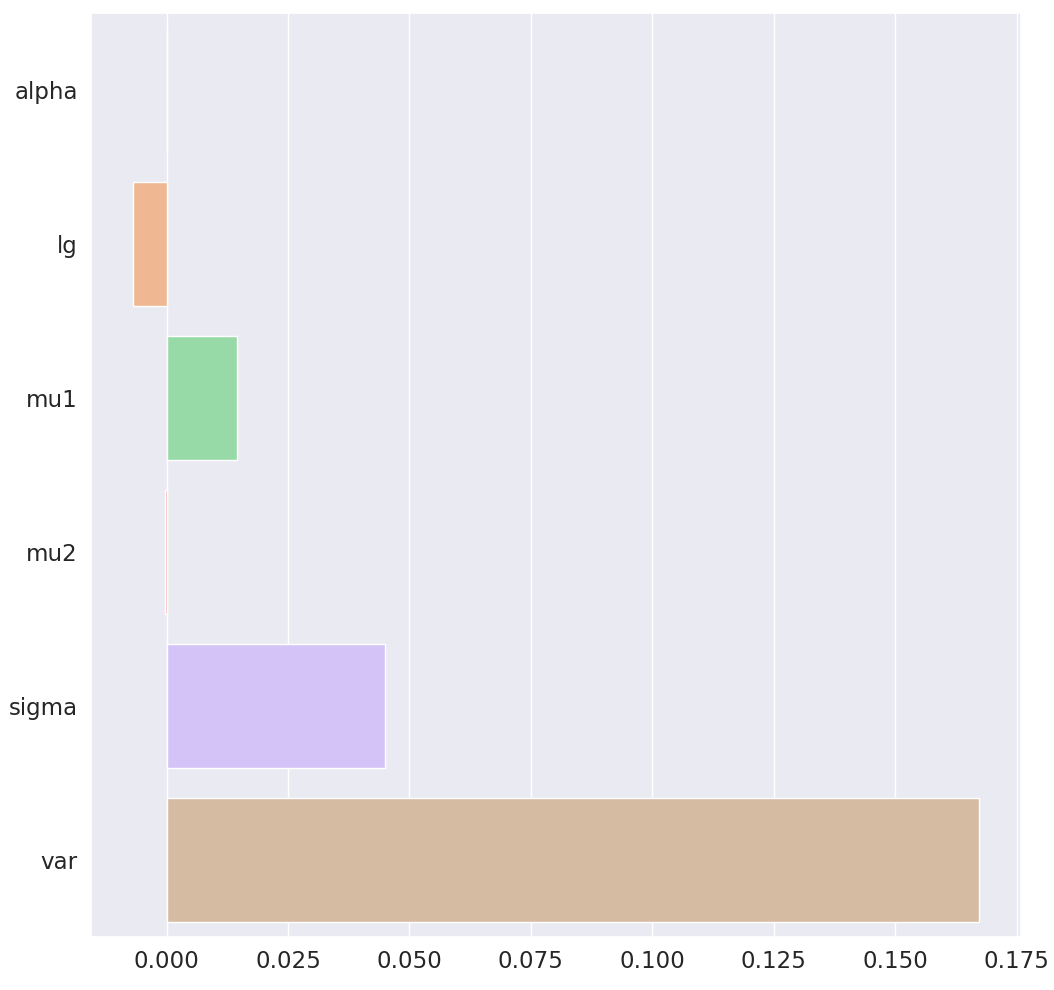
\includegraphics[scale=0.4]{feat_lr.png}
	\caption{Значимость признаков для LinearRegression}
	\label{feat_lr}
\end{figure}
На рисунке \ref{feat_lr} видно, что для алгоритма LinearRegression значимыми признаками являются задержка заявок на орбите и коэффициент вариации входящего потока. В меньшей степени является значимой интенсивность обслуживания входящий заявок, и отрицательно сказывается на результате работы наличие признака lg.
\begin{figure}[H]
	\centering
	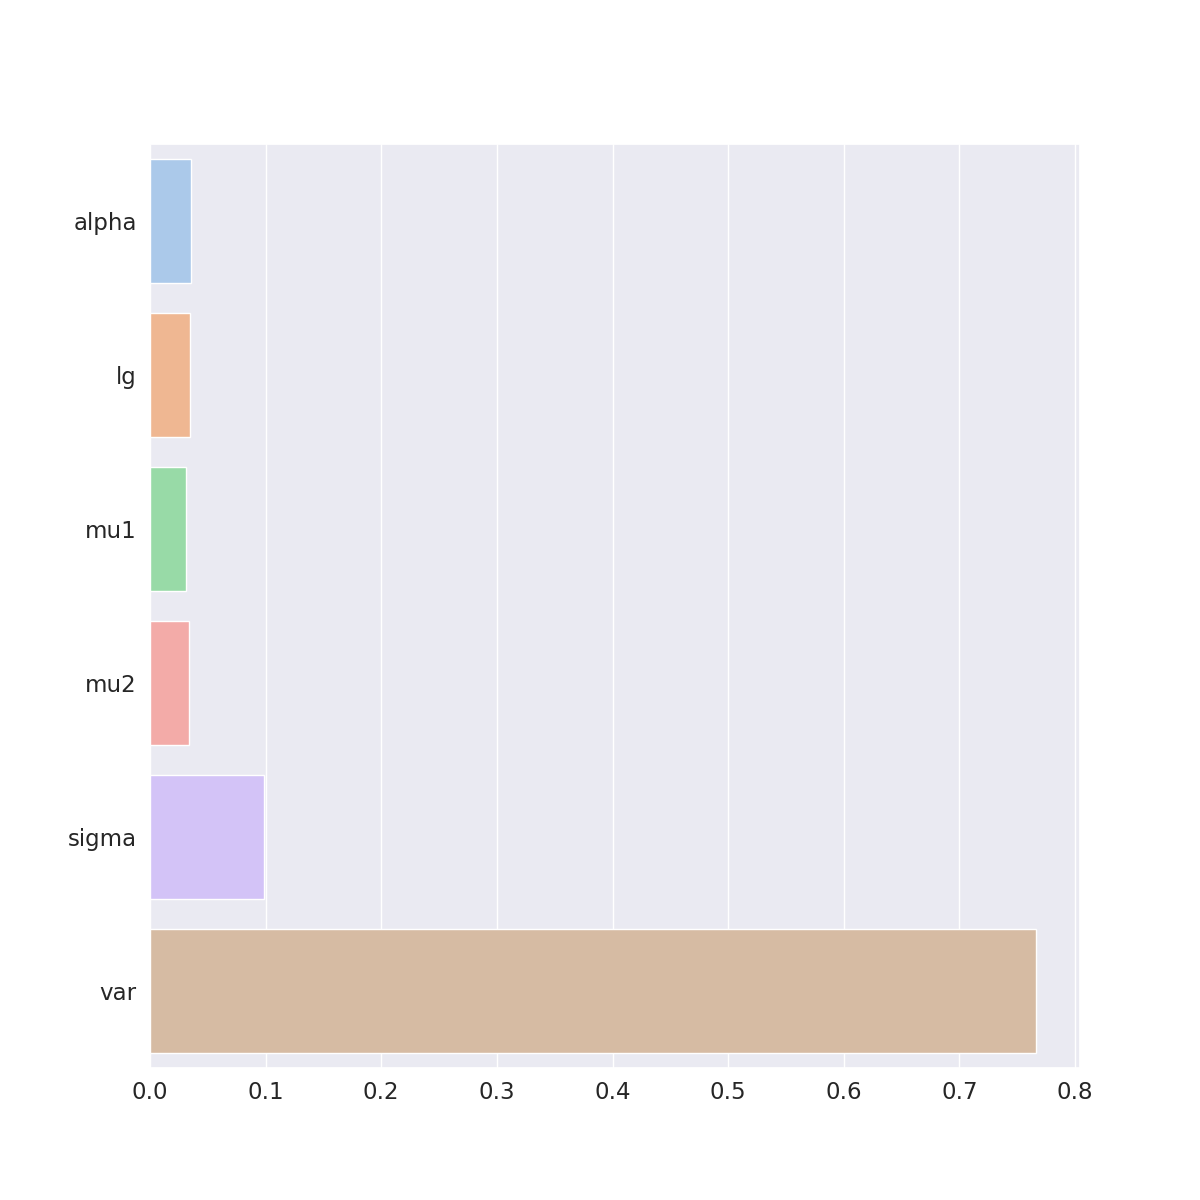
\includegraphics[scale=0.4]{feat_rf.png}
	\caption{Значимость признаков для RandomForest}
	\label{feat_rf}
\end{figure}
На рисунке \ref{feat_rf} можно наблюдать, что для алгоритма RandomForest наиболее значимыми оказались также вариация входящего потока и задержка заявок на орбите.
\begin{figure}[H]
	\centering
	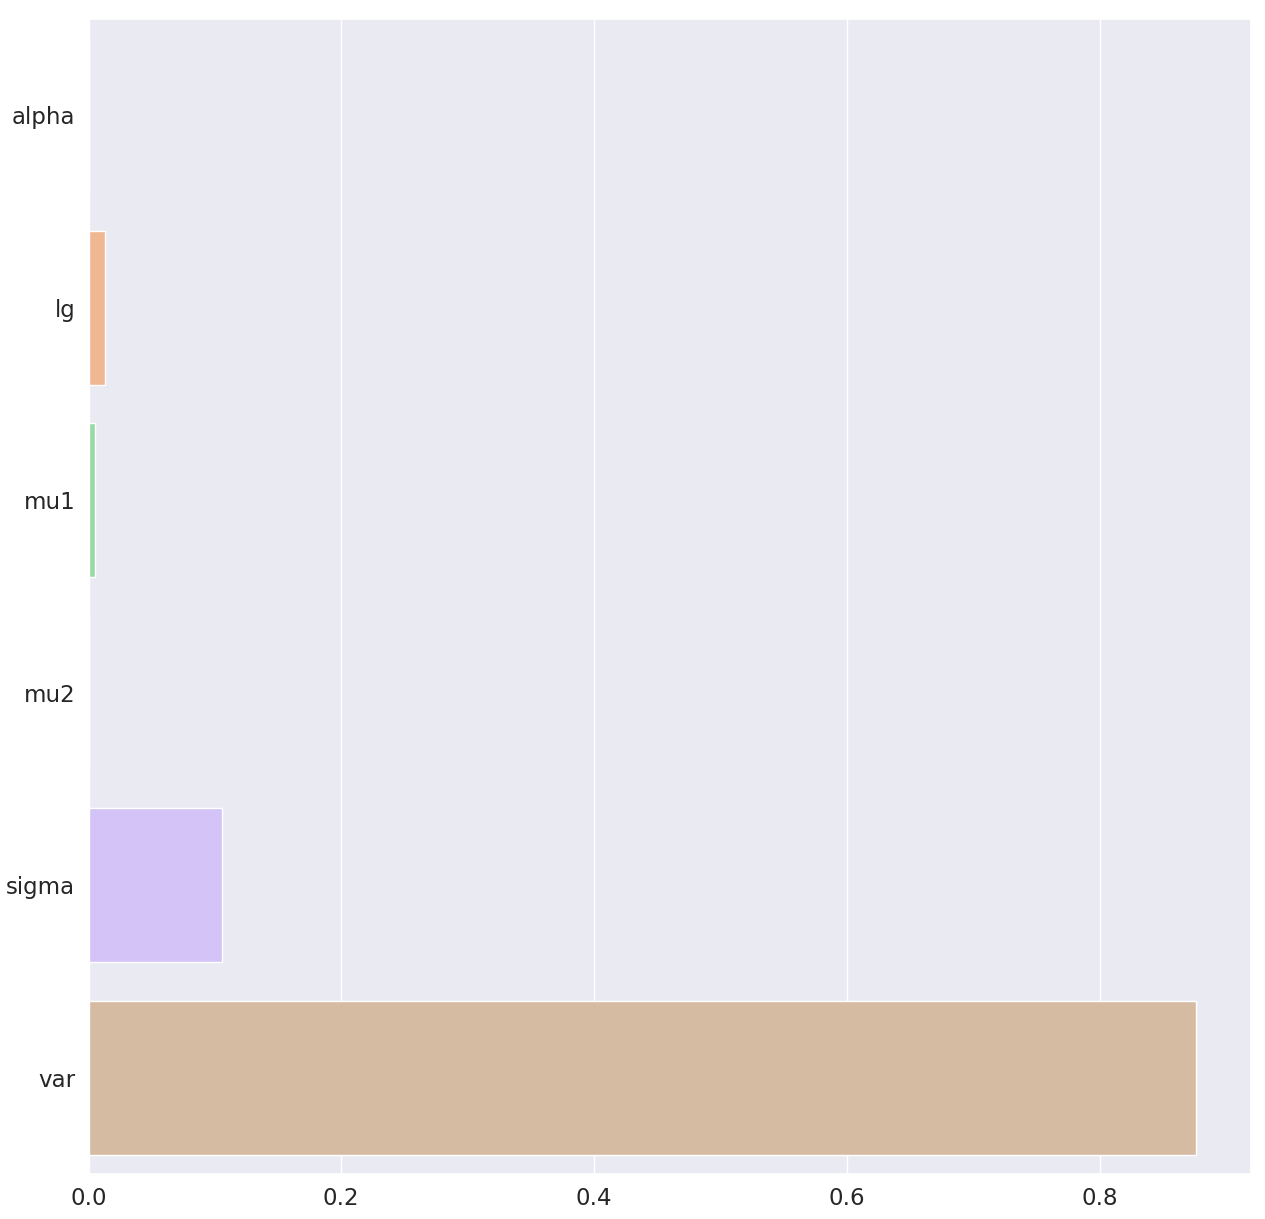
\includegraphics[scale=0.3]{feat_gb.png}
	\caption{Значимость признаков для GradientBoost}
	\label{feat_gb}
\end{figure}
\begin{figure}[H]
	\centering
	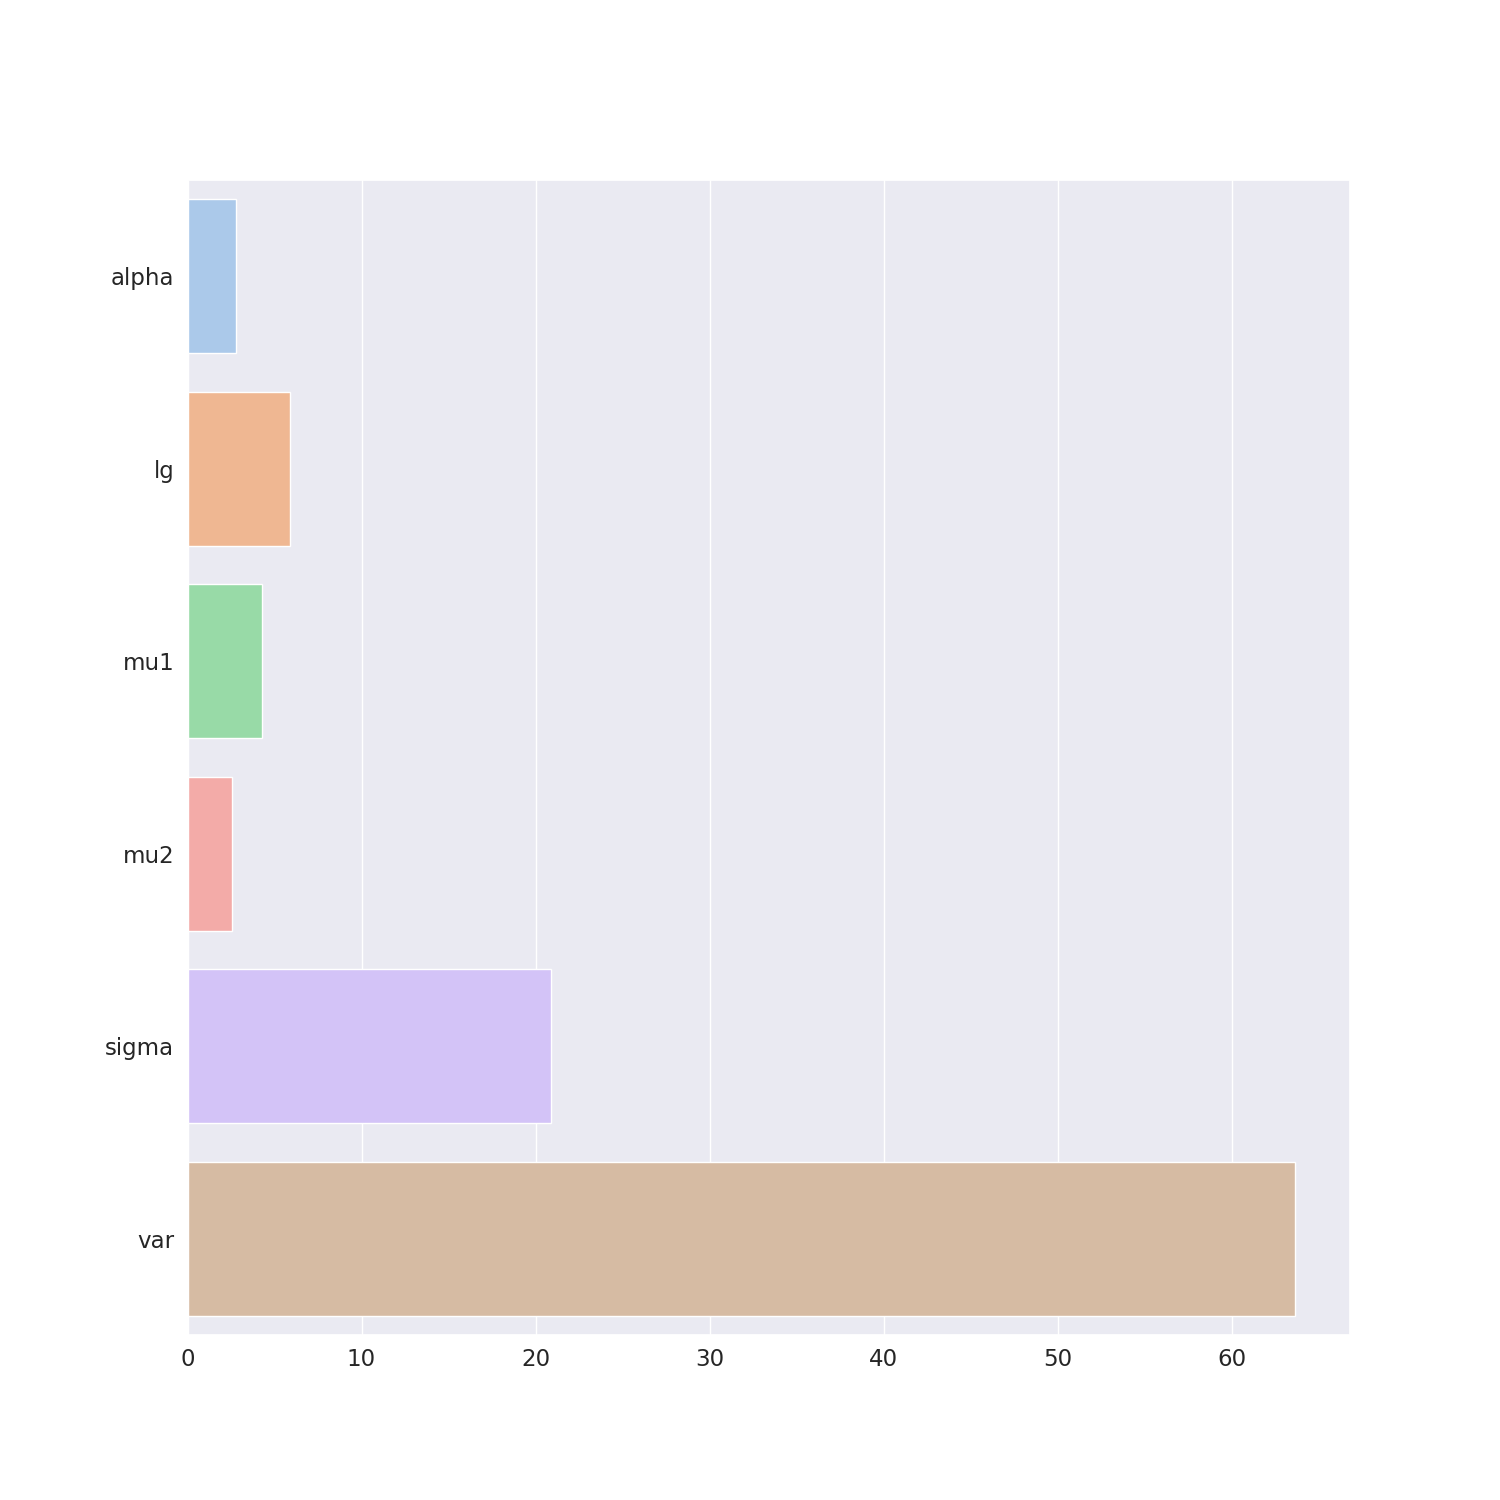
\includegraphics[scale=0.3]{feat_cb.png}
	\caption{Значимость признаков для CatBoost}
	\label{feat_cb}
\end{figure}
Для алгоритмов GradientBoost и CatBoost значимыми признаками также выступают sigma и var. Основываясь на полученных данных, оставим в обучающей выборке для каждой модели только значимые признаки.

Задание гиперпараметров алгоритмов \cite{feurer2019hyperparameter} будем производить случайным подбором в 5 итераций при помощи алгоритма scikit-learn RandomizedSearchCV. Важно заметить, что из тестовой выборки не выделялась валидационная, так как RandomizedSearchCV содержит встроенную кросс-валидацию. Он позволяет, начиная с указанных начальных значений, итеративно подобрать оптимальные гиперпараметры для модели. Для метода наименьших квадратов эта процедура не производится, поскольку метод не допускает задания каких-либо параметров.
\begin{pyin}[rand_forest_param]
rf = RandomForestRegressor(n_jobs=-1)
parameters_rf = {'n_estimators': range (100,150, 10),
    'criterion':  ['squared_error'],
    'max_depth' : range(1,9,1),
    'min_samples_split': range(2,30,5),
    'min_samples_leaf':range(1,30,5)
}
search_rf = RandomizedSearchCV(rf, parameters_rf,n_jobs=-1, n_iter = 5)
search_rf.fit(x_train_rf, y_train)
search_rf.best_params_, search_rf.best_score_
\end{pyin}
\begin{pyprint}
({'n_estimators': 110,
    'min_samples_split': 2,
    'min_samples_leaf': 26,
    'max_depth': 7,
    'criterion': 'squared_error'},
0.7699992121816944)
\end{pyprint}
\begin{pyin}[random_forest_learn]
best_model_rf = search_rf.best_estimator_
best_model_rf.fit(x_train_rf, y_train)
y_pred_test_rf = best_model_rf.predict(x_test_rf)

print('MAE:', mean_absolute_error(y_test, y_pred_test_rf))
print('RMSE:', mean_squared_error(y_test, y_pred_test_rf, squared=False))
print('R2_score:', r2_score(y_test, y_pred_test_rf))
\end{pyin}
\begin{pyprint}
MAE: 0.06538199710376982
RMSE: 0.09781859274247506
R2_score: 0.7695224558769049
\end{pyprint}
В ячейке \ref{rand_forest_param} производится задание начальных значений гиперпараметров для алгоритма случайных деревьев. Среди параметров:
\begin{itemize}
	\item n\_estimators --- количество деревьев решений.
	\item criterion --- методы оценки ошибки в процессе обучения. По умолчанию выбрано среднеквадратическое отклонение.
	\item max\_depth --- максимальная глубина дерева.
	\item min\_samples\_split --- минимальное количество сэмплов, требуемое для расщепления вершины дерева.
	\item min\_samples\_leaf --- минимальное количество сэмплов, требуемое для превращения вершины в лист.
\end{itemize}
Далее производится подбор параметров алгоритма, дающих максимальную точность, измеряемую коэффициентом детерминации. Коэффициент детерминации является основной метрикой качества для решений задач регрессии \cite{gomar2011validation}. В данном случае, он составил 0.769.
В ячейке \ref{random_forest_learn} производится обучение модели с лучшими гиперпараметрами и оценка точности, которая проводится при помощи следующих метрик:  средняя абсолютная ошибка (MAE), среднеквадратическое отклонение (RMSE) и коэффициент детерминации (R2\_score).

Для остальных моделей использовалась та же последовательность операций. В итоге, были получены следующие результаты
\begin{figure}[H]
	\centering
	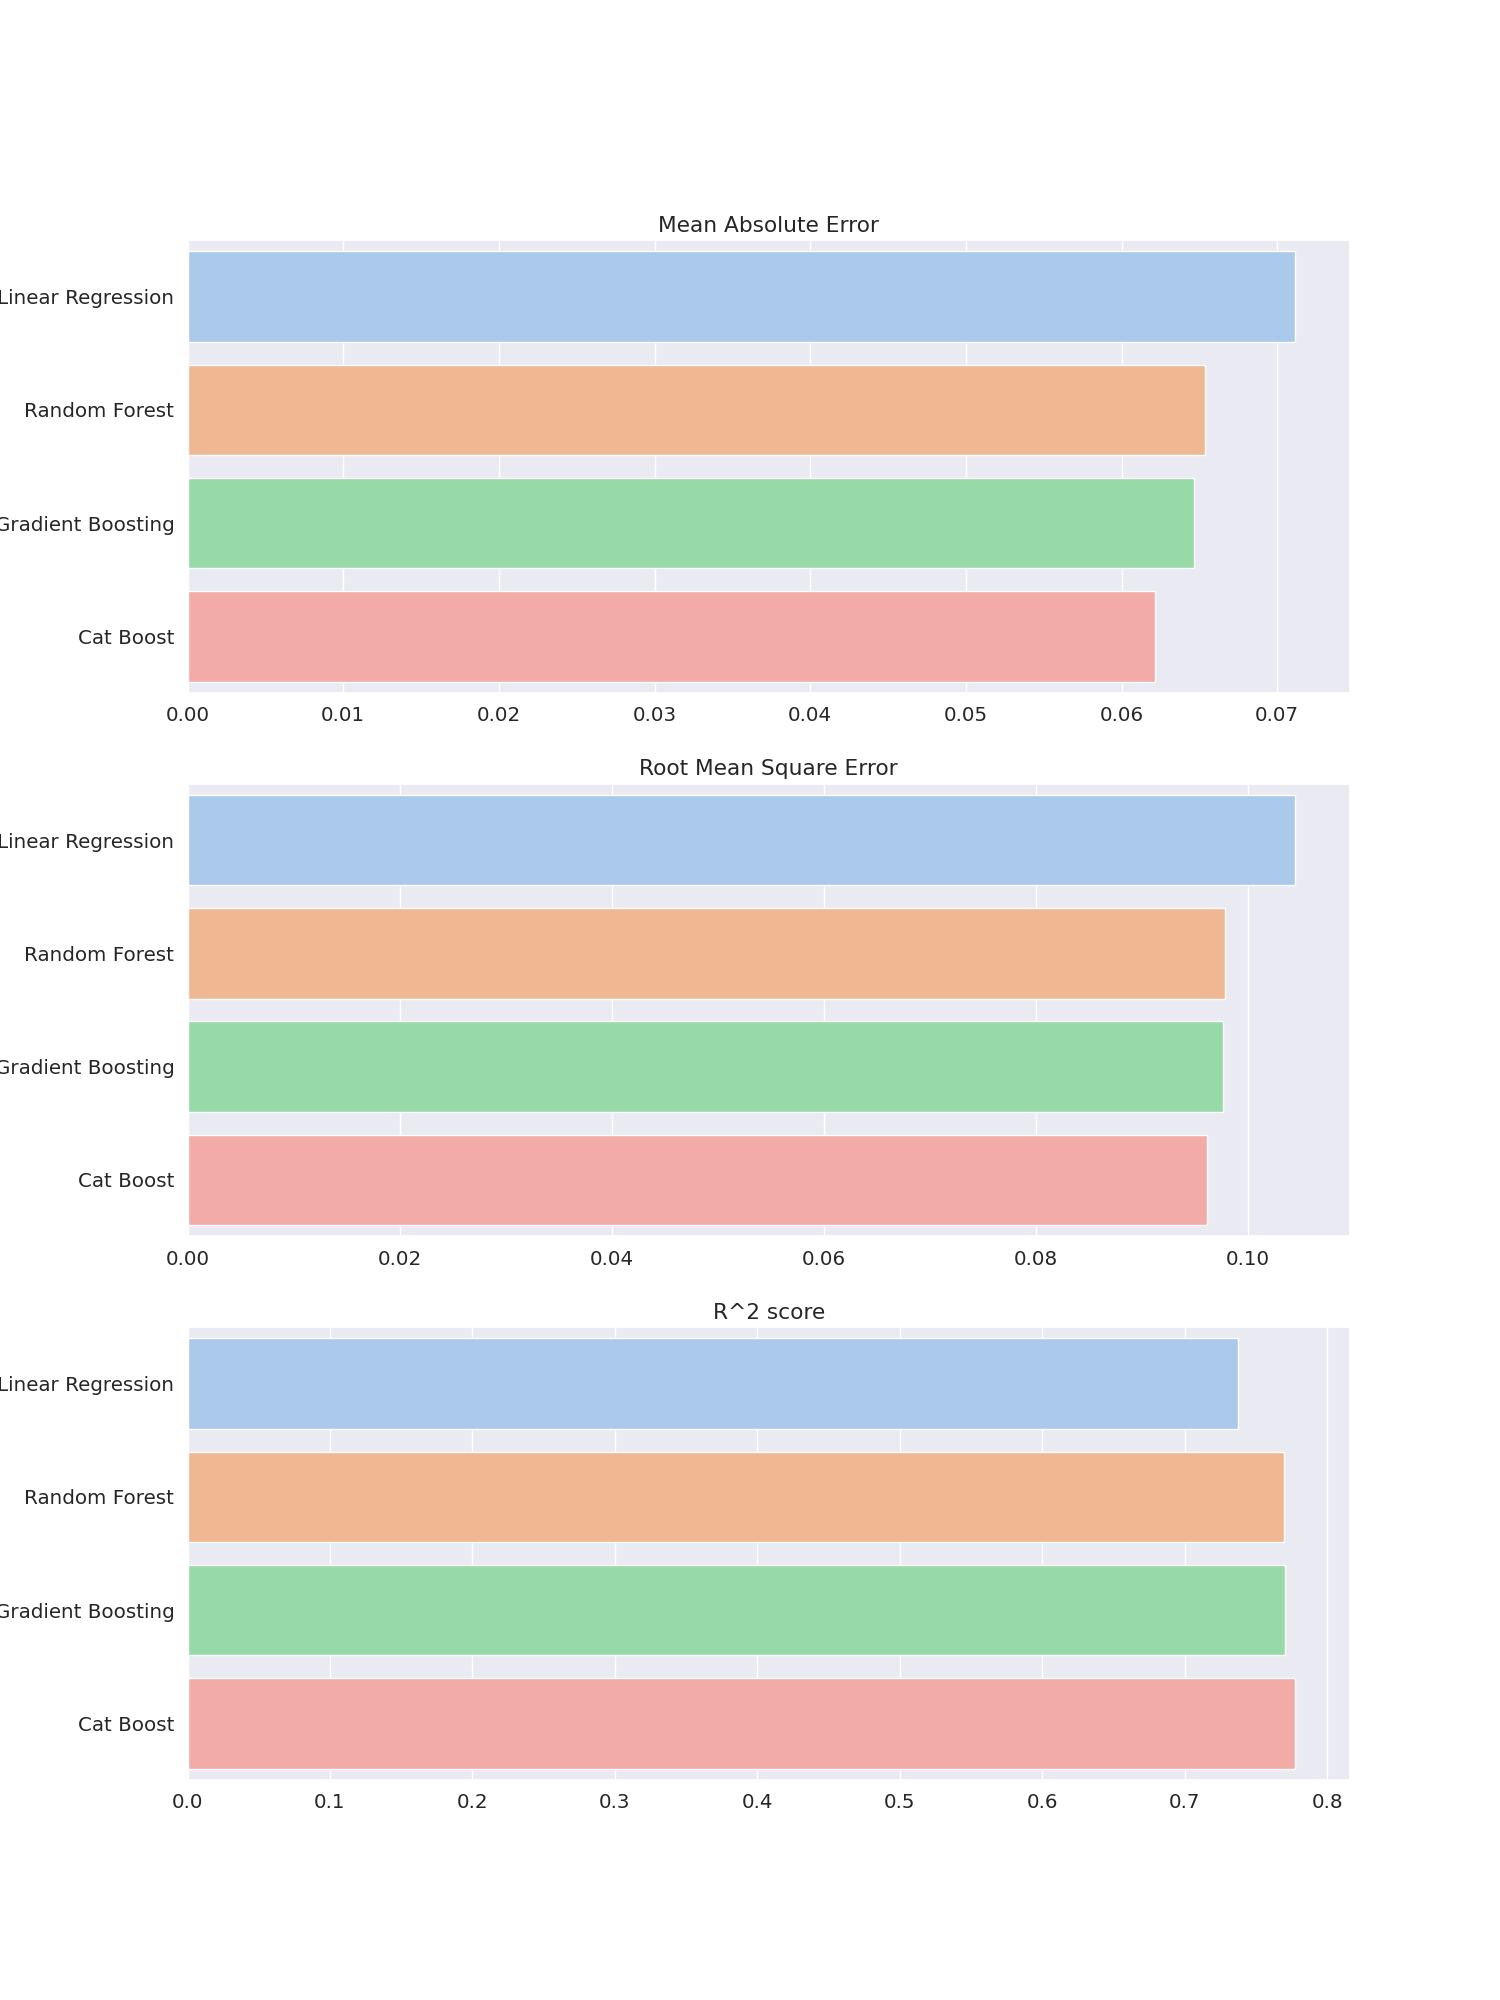
\includegraphics[scale=1,width=\textwidth]{model_accuracy.png}
	\caption{Оценка точности моделей}
	\label{model_accuracy}
\end{figure}
\begin{figure}[H]
	\centering
	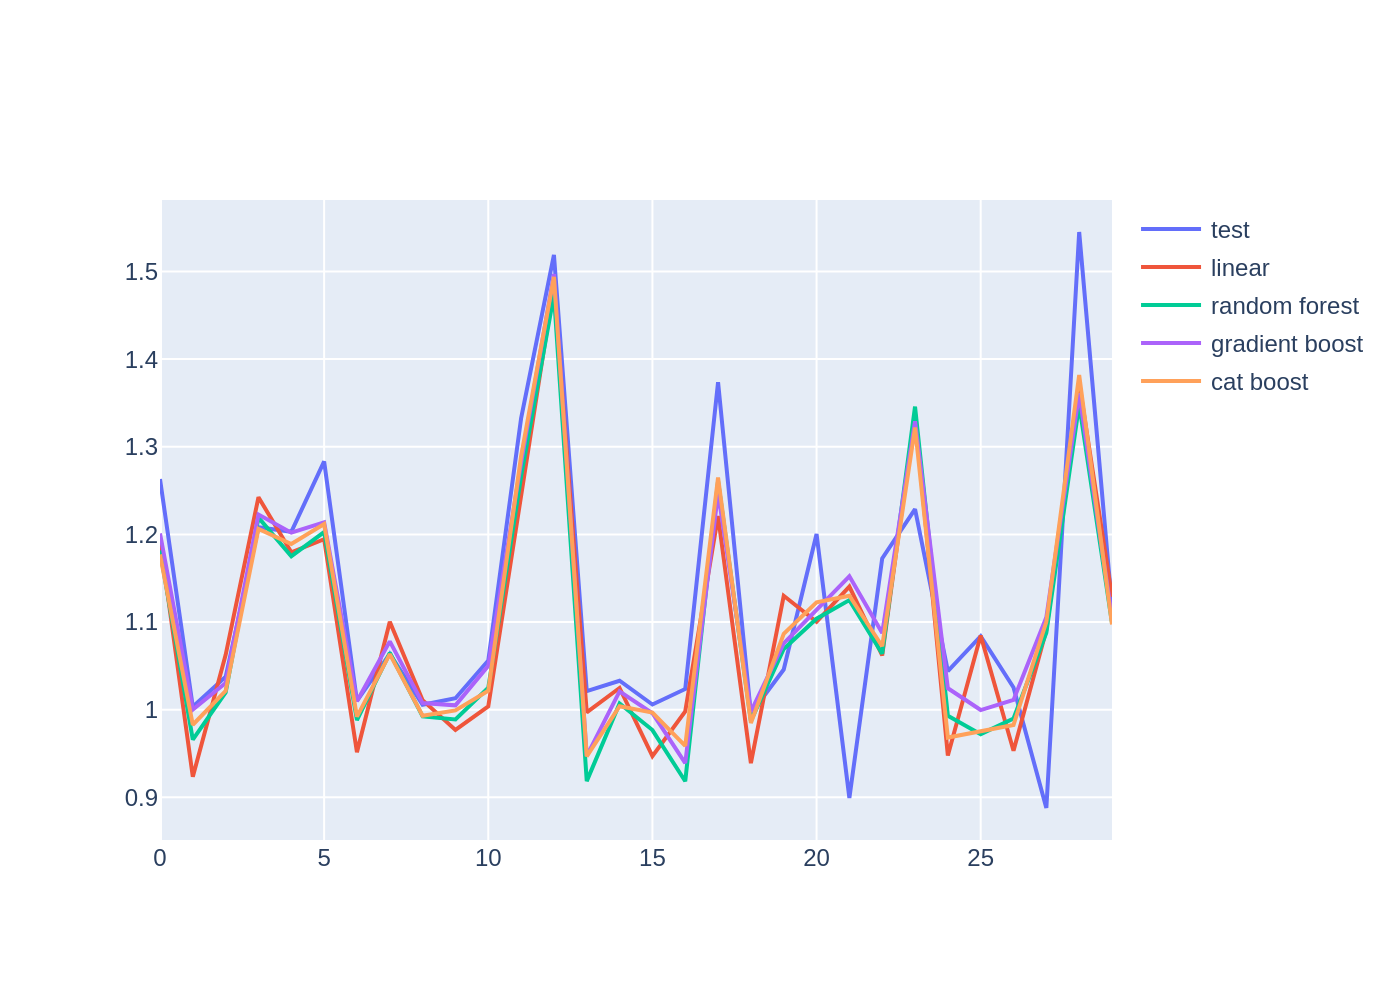
\includegraphics[scale=1,width=\textwidth]{pred_example.png}
	\caption{Сравнение предсказаний моделей}
	\label{pred_example}
\end{figure}
Как видно на рисунке \ref{model_accuracy}, CatBoost оказался самым точным среди выбранных алгоритмов --- результаты его предсказаний имеют наименьшую среднюю абсолютную и квадратические ошибки и наибольшее значение коэффициента детерминации, равное 0.774. Рассмотрение результатов предсказаний в целом показывает, что общая точность моделей находится в районе 80\%. Для апробирования подхода данный результат является в достаточной степени приемлемым. Также, можно предложить, почему точность моделей не оказалась выше: на рисунке \ref{pred_example} представлен отрезок тестового вектора значения коэффициента вариации выходящего процесса с наложением на него предсказаний. Можно заметить, что для значений, которые наиболее приближены к среднему по выборке, предсказания точны, однако для менее частых модели не смогли дать верный ответ. Это обусловлено слабой дисперсией в распределении значимых признаков в выборке (таблица \ref{table_feature_distr}), что приводит к переобучению моделей на определенном диапазоне значений признаков, делая предсказания для остальных случаев искаженными. Для улучшения качества предсказаний требуется изменить метод генерации параметров таким образом, чтобы признаки были распределены более равномерно и охватывали как можно больше возможных значений.
\clearpage